\documentclass[pdflatex,referee,sn-basic]{sn-jnl}% Basic Springer Nature reference style; referee = double spacing
% Line numbers on the text lines (lineno package). The class's own `lineno' option draws a fixed margin ruler
% at single-spacing pitch, which with double spacing gives two numbers per line and numbers beside blank space.
\usepackage[left,mathlines]{lineno}

\usepackage{graphicx}%
\usepackage{multirow}%
\usepackage{amsmath,amssymb,amsfonts}%
\usepackage{amsthm}%
\usepackage[title]{appendix}%
\usepackage{xcolor}%
\usepackage{booktabs}%
\usepackage{array}%
\usepackage{algorithm}%
\usepackage{algorithmicx}%
\usepackage{algpseudocode}%
\usepackage{tikz}
\usepackage{pgfplots}
\usepackage{scalerel}
\usetikzlibrary{positioning, decorations.pathreplacing, calligraphy, calc, shapes.geometric, intersections, arrows}
\usepgfplotslibrary{fillbetween}
\pgfplotsset{compat=1.18}

\newcommand{\fmri}{functional magnetic resonance imaging}
\newcommand{\FMRI}{Functional magnetic resonance imaging}
\newcommand{\fmriabbrv}{fMRI}
\newcommand{\eeg}{electroencephalography}
\newcommand{\EEG}{Electroencephalography}
\newcommand{\eegabbrv}{EEG}

\raggedbottom

\begin{document}
\linenumbers

\title[Benchmarking EEG-to-fMRI synthesis for diagnosis]{What Does EEG-to-fMRI Synthesis Add to EEG-Based Diagnosis? A Controlled Benchmark in Psychosis, Schizophrenia and Parkinson's Disease}

\author*[1]{\fnm{David} \sur{Calhas}}\email{davidcalhas@gmail.com}
\author[2]{\fnm{Rui} \sur{Henriques}}\email{rmch@tecnico.ulisboa.pt}

\affil*[1]{\orgdiv{Faculty of Computer and Information Science}, \orgname{University of Ljubljana}, \orgaddress{\city{Ljubljana}, \country{Slovenia}}}
\affil[2]{\orgdiv{INESC-ID, Instituto Superior T\'{e}cnico}, \orgname{Universidade de Lisboa}, \orgaddress{\city{Lisbon}, \country{Portugal}}}

\abstract{\textbf{Background:} Synthesis of functional magnetic resonance imaging (fMRI) from electroencephalography (EEG) has been proposed to support EEG-only diagnosis, but whether synthesized fMRI adds information beyond the EEG it is computed from has not been tested with appropriate controls.

\textbf{Methods:} Four synthesizers were trained on two simultaneous EEG-fMRI datasets of healthy adults and applied to resting EEG from five public cohorts: two first-episode psychosis samples (77 and 61 participants), chronic schizophrenia (77), Parkinson's disease (50) and a task-EEG schizophrenia-spectrum sample (43). Synthesized fMRI was compared with EEG band power and with an EEG view matched in information to the synthesizer input, alone and combined, under nested repeated cross-validation, permutation tests and Holm-corrected paired bootstrap; untrained (random-weight) synthesizers controlled for architecture.

\textbf{Results:} Band power separated Parkinson's disease from controls (area under the ROC curve, AUC, 0.79) but not the psychosis or schizophrenia cohorts (0.54--0.65); the information-matched view reached 0.83. Synthesized views classified Parkinson's disease (best AUC 0.74), but untrained synthesizers matched them (0.69--0.74) and no trained synthesizer added to the information-matched view in any cohort. The only gain surviving correction came from an untrained network in chronic schizophrenia and disappeared after ocular-artefact removal. The synthesizers did not outperform an EEG-free template image, and EEG explained a negligible part of the blood-oxygen-level-dependent signal (correlation 0.03).

\textbf{Conclusions:} Current synthesized fMRI is a transform of EEG spectra whose learned mapping added no diagnostic information. The protocol, code and checklist of controls set a baseline for future diagnostic claims.}

\keywords{Electroencephalography, EEG-to-fMRI synthesis, Functional MRI, Schizophrenia, First-episode psychosis, Parkinson's disease, Diagnostic classification, Cross-modal generation, Benchmark, Evaluation protocol}

\maketitle

\section{Introduction}\label{section:introduction}

fMRI resolves brain activity in space but is costly and scarce, especially in low-resource settings \cite{ogbole2018survey}; EEG is cheap and portable but spatially coarse. EEG-to-fMRI synthesis learns, from simultaneous recordings, a mapping from scalp EEG to BOLD volumes, and has been proposed as a way to obtain fMRI-like information where only EEG is available \cite{liu2019convolutional, liu2020latent, bricman2021eeg2fmri, calhas2022eeg, roos2025brainwaves, he2025spec2vol, lanzino2024ntvit, li2024neurobolt}. Schizophrenia and related psychotic disorders are a natural target: they are clinically heterogeneous \cite{saha2005systematic}, their diagnosis draws on psychological, neuroimaging, molecular and speech-based assessments \cite{andreou2020structural,neale2015genetic,corcoran2020language}, and both EEG \cite{tan2016eeg,aydin2018cortical,roach2008event,bates2009low} and fMRI \cite{oh2020identifying, velakoulis2006hippocampal, haukvik2013schizophrenia} carry group differences. Parkinson's disease, with well-documented resting EEG alterations, offers a second target. Two studies have classified patients from synthesized fMRI: schizophrenia from a task-EEG cohort, in an earlier version of this work \cite{calhas2023medrxiv}, and Parkinson's disease from eight subjects of a resting-EEG cohort \cite{yao2025catd}.

A synthesizer cannot create information that is absent from its EEG input. Its potential value for diagnosis lies instead in representation: a mapping learned from simultaneous recordings could act as a prior that reorganises EEG spectra into a space in which group differences become linearly accessible to a classifier trained on the 50--80 subjects of a typical clinical cohort. Testing this hypothesis requires controls that, to our knowledge, have not been applied together: classification data without acquisition differences between groups; a comparison, under identical validation, with EEG-only views, including one that receives the same spectral information as the synthesizer, and with the combination of EEG and synthesized views; and a test of whether any gain comes from the learned EEG-to-fMRI mapping or from the inductive bias of the architecture alone, obtained by applying the same networks with untrained weights. We report such an evaluation across four synthesizers, trained on two simultaneous EEG-fMRI datasets, and five clinical cohorts.

\textbf{Contributions.} (1) An evaluation protocol for diagnostic claims from synthesized fMRI: a harmonisation pipeline that maps any clinical EEG onto the synthesizers' training montage and removes non-EEG channels by type; EEG-only baselines, including one matched in information to the synthesizer input, and fusion tests under identical nested validation; untrained-network controls; artefact and recording-condition checks; and subject-level permutation and corrected paired bootstrap inference. (2) A benchmark applying this protocol to four synthesizers (the convolutional neural network with topographical attention graph, CNN-TAG \cite{calhas2022eeg}, E2fNet, Spec2VolCAMU-Net and NT-ViT), trained on two simultaneous EEG-fMRI datasets, and to a contrastive fine-tuning method \cite{calhas2023medrxiv} on five public cohorts spanning first-episode psychosis, chronic schizophrenia, a schizophrenia-spectrum task cohort and Parkinson's disease. (3) Supporting evidence on what the synthesizers learn: a scanner-trigger-aligned training protocol for the NODDI dataset, an EEG-free template baseline and a fair-target test of how much BOLD variance EEG predicts. (4) A checklist of controls for diagnostic uses of synthesized fMRI (Section~\ref{section:discussion}), with open code. In brief, the synthesized volumes were transforms of the EEG spectra they are computed from: no trained synthesizer added diagnostic information to an EEG view matched in information, and the one gain that survived correction came from an untrained network and disappeared after ocular-artefact removal.

\section{Related work}\label{section:related_work}

\noindent\textbf{EEG-to-fMRI synthesis.} Convolutional transcoders \cite{liu2019convolutional, liu2020latent}, attention- and Fourier-feature-based encoder-decoders \cite{calhas2022eeg}, U-Net and Mamba decoders \cite{roos2025brainwaves,he2025spec2vol}, vision transformers \cite{lanzino2024ntvit} and diffusion models \cite{yao2025catd} synthesize volumes, while NeuroBOLT and UnEBOLT \cite{li2024neurobolt,li2026unebolt} and distributed-lag models \cite{mehta2025time} predict region time series; the latter work showed, within subjects and with surrogate tests, that EEG predicts BOLD in task-relevant regions. Downstream diagnostic use has been reported for schizophrenia \cite{calhas2023medrxiv} and Parkinson's disease \cite{yao2025catd}.

\noindent\textbf{Schizophrenia.}\label{related_work:schizophrenia} Schizophrenia is marked by cognitive and structural brain alterations \cite{sui2018multimodal}. fMRI-based classification of controls and patients has shown promise \cite{de2019machine}, with consistent findings of frontal and temporal volume reductions \cite{chin2018recognition} and white-matter abnormalities \cite{cetin2020white}. EEG-based classification is common, but its pitfalls, including small samples and validation that is not at the subject level, have been documented \cite{barros2021advanced}; acquisition differences between groups in public releases are a further risk.

\noindent\textbf{Interpretability.}\label{related_work:interpretability} For EEG, interpretability remains a challenge. \citet{pinto2022interpretable} applied evolutionary feature selection and \textit{apriori} association rules to explain seizure detection, identifying key features across spectral, temporal, and electrode dimensions. Band power, used here as the EEG baseline, is itself spatially organised over the scalp and has established clinical interpretations in schizophrenia \cite{roach2008event,bates2009low}; the case for synthesized fMRI as a more interpretable view would require spatial maps validated against real fMRI in patients, which the present data cannot provide.

\section{Materials and methods}\label{section:methods}

Figure~\ref{fig:overview} summarises the study design.

\begin{figure*}[!htbp]
    \centering
    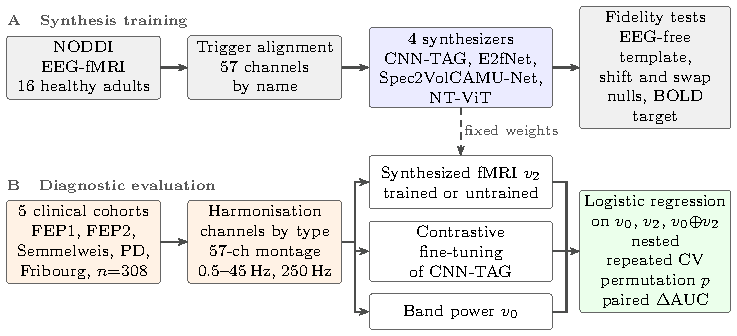
\includegraphics[width=\textwidth]{fig1.pdf}
    \caption{\textbf{Study design.} Four synthesizers are trained on simultaneous EEG-fMRI of healthy adults (NODDI) with scanner-trigger alignment and kept fixed. Resting EEG of five clinical cohorts is harmonised to the training montage and represented by band power ($v_0$), by the synthesized fMRI of each synthesizer with learned or random weights ($v_2$), and by their combination ($v_0\oplus v_2$); a contrastive fine-tuning of CNN-TAG is evaluated alongside. Every view is classified with the same nested cross-validation and permutation tests. Supporting analyses on NODDI test what the synthesizers learn.}
    \label{fig:overview}
\end{figure*}

\subsection{Datasets}\label{materials:data}

Table~\ref{tab:data_description} summarises the datasets. All are previously published, anonymised public releases analysed here as secondary data.

\noindent\textbf{First-episode psychosis (FEP1, FEP2).} Two independently collected samples from the University of Pittsburgh (OpenNeuro ds003944 and ds003947) \cite{salisbury_ds003944,salisbury_ds003947}: individuals with a first episode of psychosis and healthy controls; five minutes of eyes-open resting EEG recorded with a 10-10 cap inside an Elekta Neuromag Vectorview MEG system (61 EEG channels, 1000\,Hz, reference TP9). Age, sex, symptom and functioning scales (BPRS, SANS, SAPS, GAF, SFS), cognition (MATRICS, WASI) and chlorpromazine-equivalent medication are released. FEP1 lists 82 recordings, but five people appear twice under the identifiers \texttt{sub-X} and \texttt{sub-XA} (same age, sex and race, recorded days apart); we kept one recording per person (47 patients, 30 controls). FEP2 contains 31 patients and 30 controls and excludes, by construction, the subjects shared with FEP1.

\noindent\textbf{Chronic schizophrenia (Semmelweis).} Resting EEG from Semmelweis University, Budapest \cite{racz2025}: 38 patients with schizophrenia and 39 age- and sex-matched controls; about two minutes of eyes-closed rest, 64-channel Neuroscan amplifier at 1000\,Hz. Patients are identified by the presence of PANSS ratings, which reproduces the 38/39 split of the source publication (35 of the 38 carry an ICD-10 F20/F25 code in the released table; three have a missing or non-F2 code). Medication, illness duration, education and PANSS scores are released.

\noindent\textbf{Parkinson's disease (PD).} Resting EEG from the University of New Mexico (OpenNeuro ds003490) \cite{cavanagh_ds003490}: 25 patients with Parkinson's disease and 25 matched controls; 63 EEG channels, 500\,Hz (Brain Vision ActiChamp; reference CPz), instructed one-minute eyes-closed and eyes-open spans, followed in the same file by an auditory oddball task (Section~\ref{section:adaptation}), plus EOG and a three-axis accelerometer on the most tremor-affected hand. Patients were recorded twice, a week apart, ON and OFF dopaminergic medication (13 ON first, 12 OFF first); we analysed the OFF session. Eight subjects of this cohort were used by \cite{yao2025catd}.

\noindent\textbf{Schizophrenia spectrum, task EEG (Fribourg).} The cohort used in \cite{calhas2023medrxiv}, released by \cite{dataset2022fribourg}: 19 patients with a psychotic disorder (ICD-10) and 24 controls, recorded during the Ultimatum Game (responder role), 128-channel Biosemi ActiveTwo at 2048\,Hz; the release includes additional EXG channels whose layout differs between groups (four in all controls, six in 18 of 19 patients), which are excluded by the channel selection of Section~\ref{section:adaptation}. The public release distributes the group label only; group-level characteristics are reported in \cite{horat2018impaired}.

\begin{table}[!htbp]
    \centering
    \caption{Characteristics and roles of the datasets. \textit{pt}: patients; \textit{hc}: healthy controls; age as mean $\pm$ standard deviation (years); analysed EEG is the fixed crop used for every subject of a cohort.}
    \label{tab:data_description}
    \small
    \begin{tabular}{p{1.75cm} | p{1.95cm} | p{0.85cm} | p{2.0cm} | p{1.3cm} | p{2.65cm}}
        \hline
        \hline
         \hfil Dataset & \hfil Role / disease & \hfil pt/hc & \hfil Age pt | hc & \hfil Sex (M/F) pt | hc & \hfil Recording (analysed EEG) \\
         \hline
         NODDI & synthesis training & 0/16 & \hfil $32.8\pm8.1^{a}$ & \hfil 11/6$^{a}$ & rest, eyes open, simultaneous EEG-fMRI, 64 ch, 250\,Hz \\
         FEP1 (ds003944) & first-episode psychosis & 47/30 & $22.5\pm5.1$ | $21.6\pm4.1$ & 33/14 | 18/12 & rest, eyes open, 61 ch, 1\,kHz (300\,s) \\
         FEP2 (ds003947) & first-episode psychosis & 31/30 & $23.4\pm4.7$ | $24.2\pm5.1$ & 22/9 | 16/14 & rest, eyes open, 61 ch, 1\,kHz (300\,s) \\
         Semmelweis & schizophrenia (chronic) & 38/39 & $33.9\pm10.6$ | $32.7\pm9.7$ & 24/14 | 24/15 & rest, eyes closed, 64 ch, 1\,kHz (118\,s$^{b}$) \\
         PD (ds003490) & Parkinson's disease (OFF) & 25/25 & $69.7\pm8.7$ | $69.3\pm9.6$ & 16/9 | 16/9 & rest, eyes closed/open spans, 63 ch, 500\,Hz (400\,s) \\
         Fribourg (ds004000) & schizophrenia spectrum & 19/24 & n/a & n/a & Ultimatum Game, 128 ch, 2048\,Hz (400\,s) \\
         \hline
         \hline
    \end{tabular}

    \raggedright\footnotesize $^{a}$For the 17 acquired participants; version 2 of the release contains 16. $^{b}$One control recording is 109.7\,s long and was used in full.
\end{table}

\noindent\textbf{Data checks.} For every cohort we checked for repeated participants, verified group sizes against the source publications, and tested whether recording metadata (channel set, sampling rate, filters, duration, recording date and hour, file size) differs between groups; fixed-length crops remove duration differences.

\subsection{Simultaneous EEG-fMRI for synthesis (NODDI)}\label{section:fmri_data}

fMRI is available only in the synthesis training dataset, NODDI \cite{dataset_01,deligianni2016}; the clinical cohorts are EEG-only and contain no fMRI. In NODDI, fMRI was acquired simultaneously with EEG at rest (eyes open, fixation) on a 1.5\,T Siemens Avanto: T2*-weighted gradient-echo EPI, TR/TE 2160/30\,ms, 30 slices of 3\,mm (1\,mm gap), effective voxel size $3.3\times3.3\times4.0$\,mm, $64\times64\times30$ voxels, 300 volumes; EEG with a 64-channel MR-compatible cap (BrainCap MR), recorded at 5\,kHz, released at 250\,Hz after artefact correction.

Two properties of this release matter for synthesis and, to our knowledge, have not been reported. First, in 15 of the 16 subjects the EEG begins 13--130\,s before the first fMRI volume; pairing EEG and fMRI from the start of the file would pair EEG with volumes 6--60 TRs away. We pair them through the scanner volume markers in the EEG file (one per TR). Second, two electrode montages are present: 10 subjects have F1/F2/C1/C2/P1/P2 and 6 have P9/P10/PO9/PO10/O9/O10, in a different channel order, so positional channel indexing mixes electrodes across subjects. We use the 57 channels recorded in all subjects, selected by name; the ECG channel is excluded.

\subsection{EEG harmonisation and preprocessing}\label{section:adaptation}

EEG datasets differ in electrode count and layout, sampling rate, reference and paradigm, which changes their representation in $\mathbb{R}^{C \times T}$. We apply a single harmonisation to every recording, clinical or not, so that each synthesizer receives inputs in exactly the montage and sampling rate it was trained on:

\noindent\textbf{Channel selection by type.} EEG channels are selected by their declared type, never by position; EOG, ECG, EMG, accelerometer, trigger and auxiliary (EXG) channels are removed. Selection by type also keeps acquisition differences unrelated to the disease out of the input: in the Fribourg release, for example, the auxiliary (EXG) channel layout differs between patients and controls.

\noindent\textbf{Montage harmonisation.} Channels are mapped to standard 10-05 positions and interpolated with spherical splines onto the 57 EEG channels recorded in every NODDI subject (Section~\ref{section:fmri_data}).

\noindent\textbf{Common filtering and resampling.} Notch filtering at the mains frequency and harmonics, 0.5--45\,Hz band-pass, average reference and resampling to 250\,Hz. Frequencies above 45\,Hz are discarded for every dataset, so all synthesizers see the same frequency range.

Clinical EEG has no fMRI volume markers; the synthesizers are applied to consecutive pseudo-TRs of 2.16\,s starting 43.2\,s into each recording, so that every synthesized volume has a full 20-segment history.

All recordings went through this harmonisation (MNE-Python). Each clinical recording was cropped to a fixed duration per cohort (Table~\ref{tab:data_description}), identical for patients and controls, to remove duration differences between groups. The cleaned NODDI EEG released by the dataset authors, in which scanner (gradient) and pulse (ballistocardiographic) artefacts were removed \cite{dataset_01}, was used as is before harmonisation.

\noindent\textbf{Artefact handling.} The primary analysis applies no artefact rejection or independent component analysis (ICA), so that every view receives the same input. As a sensitivity analysis, every recording was re-harmonised with ICA (FastICA, 20 components fitted on a 1\,Hz high-passed copy, before interpolation), removing the components correlated with the EOG (MNE \texttt{find\_bads\_eog}, $z>3$), using only EOG channels present in every recording of a cohort so that the cleaning could not differ by group through the channel set; all views, synthesized ones included, were then recomputed. The standard muscle criterion (\texttt{find\_bads\_muscle}) flagged most components of the 45\,Hz low-passed data and was not used for removal; muscle artefacts were instead addressed by recomputing band power without the 30--45\,Hz band. Artefact burden was compared between groups through the fraction of pseudo-TRs exceeding 150\,$\mu$V peak-to-peak or an EMG-like 30--45\,Hz power (median plus three robust standard deviations), the median peak-to-peak amplitude, the power of the EOG channels and, in Parkinson's disease, the power of the accelerometer on the most affected hand. In Parkinson's disease, the released rest file contains a set-up period, one minute of eyes closed, one minute of eyes open and then an auditory oddball task; besides the fixed 0--400\,s crop of the primary analysis, a rest-only crop from the first to the last eyes-closed or eyes-open marker was analysed, with and without ICA.

\subsection{Problem formulation and EEG views}\label{section:problem_description}

Each subject's recording, $\vec{x}_0 \in \mathbb{R}^{D_0}$, is labelled $y \in \{0,1\}$ (control or patient) and represented by views $v_i = F_i(\vec{x}_0) \in \mathbb{R}^{D_i}$, where $F_i$ is a fixed or learned transformation with parameters $\theta_i$: the band-power view $v_0$, the STFT view $v_1$ and the synthesized-fMRI view $v_2$, defined below. A view is evaluated by an $l_2$-regularised logistic regression minimising
\begin{equation}\label{equation:loss}
    \mathcal{L}_C = -\sum_{s} \left[ y_s \log \hat{p}_s + (1-y_s) \log(1-\hat{p}_s) \right] + \frac{1}{2C}\|\vec{w}\|_2^2, \qquad \hat{p}_s = \sigma\!\left(\vec{w}^\top v_i(\vec{x}_{0,s}) + b\right),
\end{equation}
over training subjects $s$, where $\vec{w} \in \mathbb{R}^{D_i}$ and $b \in \mathbb{R}$ are the classifier parameters, $\sigma$ is the logistic function and $C$ is the inverse regularisation strength. The question is whether a synthesized-fMRI view, alone or added to an EEG view, lowers the expected loss on unseen subjects relative to the EEG view alone.

\subsubsection{Band-power view}\label{eeg_views:bandpower}

Frequency-domain EEG features are long-established markers in schizophrenia and Parkinson's disease \cite{itil1977qualitative,roach2008event,bates2009low,barros2021advanced}. We use the simplest such view: for each of the $C=57$ channels (Section~\ref{section:adaptation}), Welch power spectra (4\,s windows) summarised as relative log power in five bands (1--4, 4--8, 8--13, 13--30, 30--45\,Hz), so $v_0(\vec{x}_0) \in \mathbb{R}^{C\times5}$. Band power is spatially organised over the scalp and clinically interpretable, so it is both the natural EEG-only baseline and the information any synthesized view starts from.

\subsubsection{STFT view}\label{eeg_views:channel_freq_time}

Time-frequency features are widely used in EEG studies of psychiatric and neurological disorders \cite{fingelkurts2007impaired,burgess2002functional,albrecht2018time,roach2008event,bates2009low}. The synthesizers take a short-time Fourier representation \cite{jacobsen2003sliding} as input, $\vec{x}_1 = v_1(\vec{x}_0) \in \mathbb{R}^{D_1}$, $D_1 = C \times F \times T$: log-magnitude spectra of $T=20$ consecutive EEG segments of one fMRI repetition time (TR, 2.16\,s) each, between 0.46 and 45\,Hz ($F=97$ bins), i.e. the 43.2\,s of EEG preceding an fMRI volume, which covers the haemodynamic delay. This view is the input of every synthesizer. Its temporal mean and standard deviation over a recording's pseudo-TRs (Section~\ref{section:adaptation}) also give an EEG-only view that is matched in information to the synthesized-fMRI view (Section~\ref{section:setting}).

\subsection{Synthesizers and the synthesized fMRI view}\label{eeg_views:eeg_to_fmri}

\begin{figure*}[!t]
    \centering
    \begin{tikzpicture}
        [inner sep=2mm, scale=0.87]

        \node (x) at (0,0) {};
        
        \node (stft) at ($(x)+(-1.2,0.3)$) {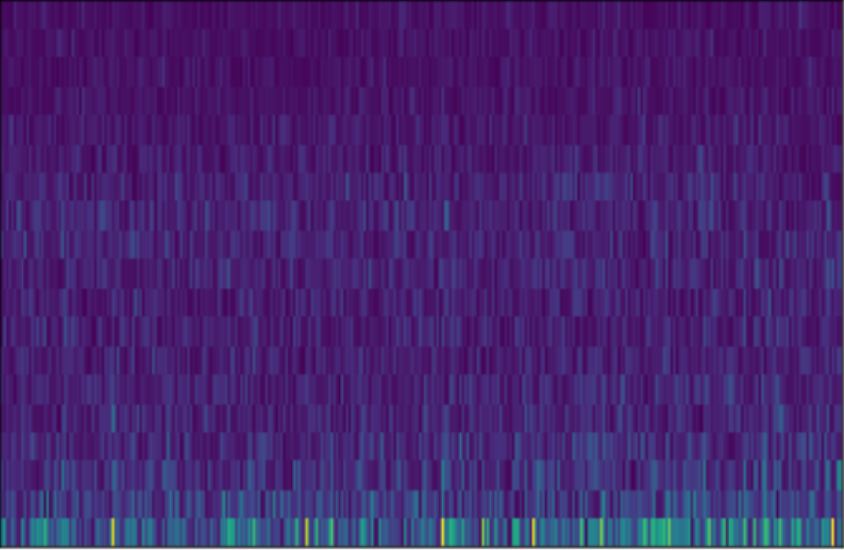
\includegraphics[width=0.1\textwidth]{stft.png}};
        \node (stft) at ($(stft)+(0.1,-0.1)$) {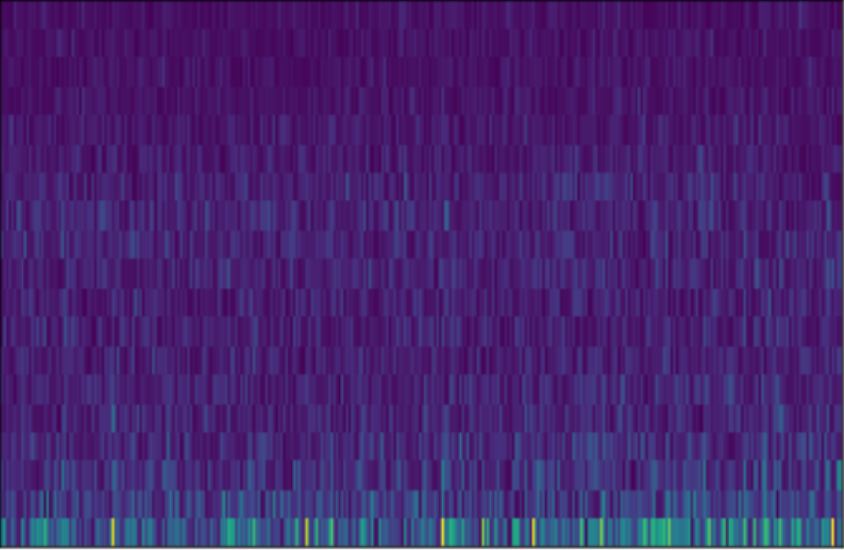
\includegraphics[width=0.1\textwidth]{stft.png}};
        \node (stft) at ($(stft)+(0.1,-0.1)$) {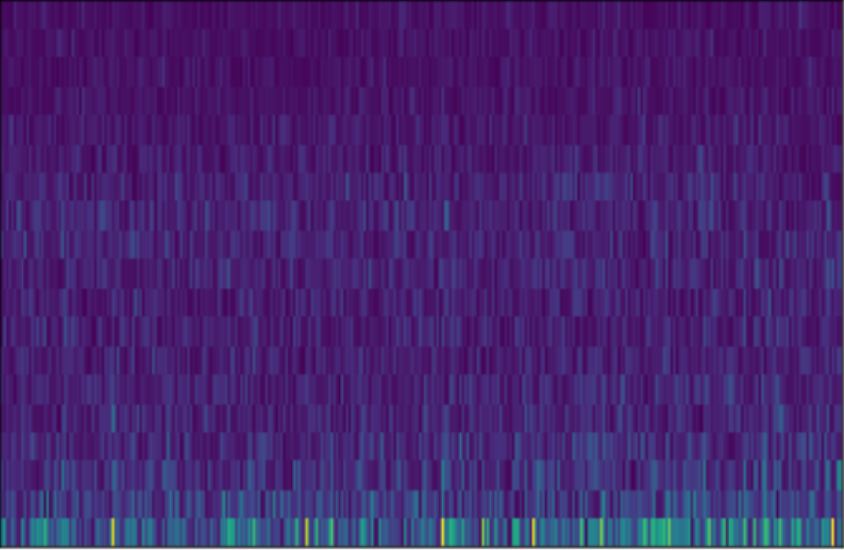
\includegraphics[width=0.1\textwidth]{stft.png}};
        \node (stft) at ($(stft)+(0.1,-0.1)$) {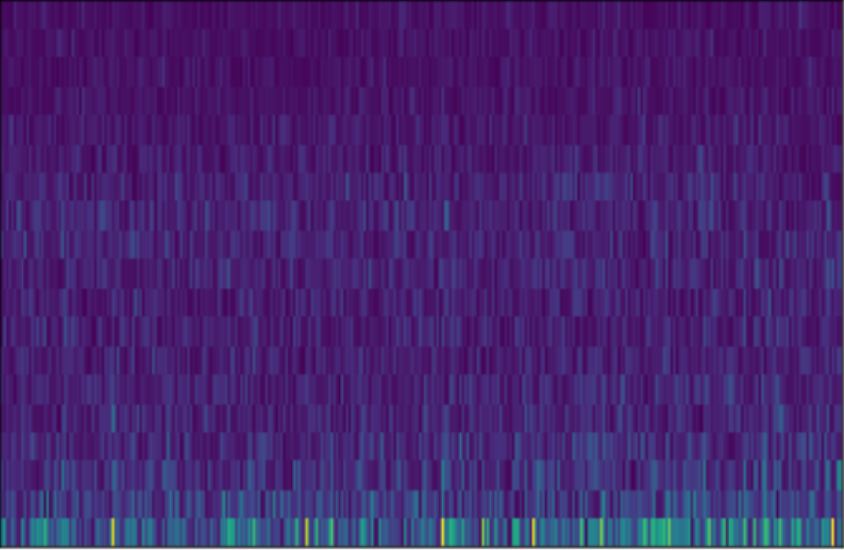
\includegraphics[width=0.1\textwidth]{stft.png}};
        \node (stft) at ($(stft)+(0.1,-0.1)$) {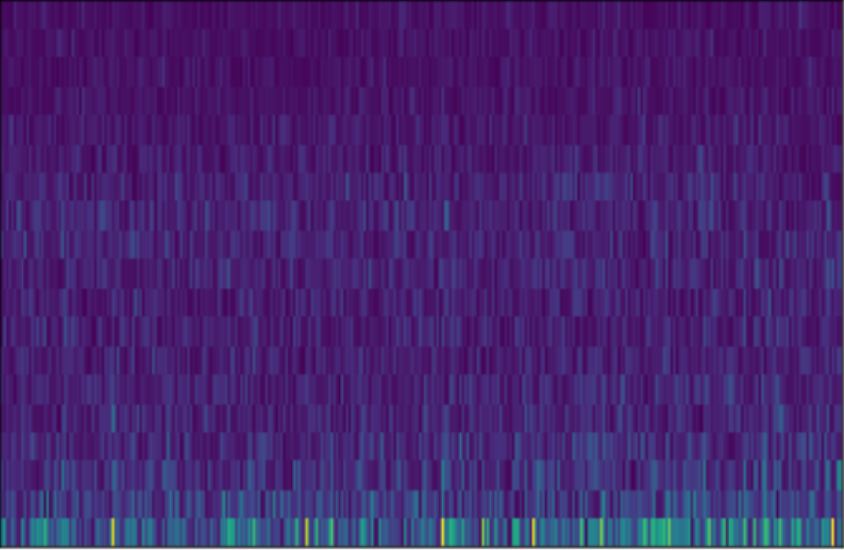
\includegraphics[width=0.1\textwidth]{stft.png}};
        
        \node at ($(stft)+(-0.2,-0.9)$) {$\vec{x}_1$};
        
        \node (encoder) at ($(x)+(2.3,0)$) {\tikz {\draw[rounded corners, draw=black!50,fill=black!20,thick, dash pattern=on 7pt off 2pt] (0,0) rectangle ++(3.4,3);}};
        \node (decoder) at ($(x)+(7.8,0)$) {\tikz {\draw[rounded corners, draw=brown!70,fill=green!20,thick, dash pattern=on 7pt off 2pt] (0,0) rectangle ++(4.5,3);}};
        \node (legend_encoder) at ($(encoder)+(0,-1.9)$) {Encoder};
        \node (legend_decoder) at ($(decoder)+(0,-1.9)$) {Decoder};
        
        
        \node (channel_organization) at ($(x)+(1,0)$) {\tikz {\draw[draw=blue!50,fill=blue!20,thick] (0,0) rectangle ++(0.3,2);}};

        \node (T) at ($(channel_organization)+(0.7,0)$) {$T$};

        \node (resblock1) at ($(T)+(0.7,0)$) {\tikz {\draw[rounded corners, draw=red!40,fill=red!20,thick] (0,0) rectangle ++(0.3,2);}};

        \node (resblock2) at ($(resblock1)+(0.7,0)$) {\tikz {\draw[rounded corners, draw=red!40,fill=red!20,thick] (0,0) rectangle ++(0.3,2);}};

        \node (latent_affine) at ($(resblock2)+(0.7,0)$) {\tikz {\draw[draw=orange!40,fill=orange!20,thick] (0,0) rectangle ++(0.3,2);}};

        \node (latent) at ($(latent_affine)+(1,0)$) {$\vec{z}$};

        \node (fourier) at ($(latent)+(2,0)$) {$cos(\omega \cdot \vec{z} + \beta)$};

        \node (style) at ($(fourier)+(2,0)$) {$\odot $};
        \node (style_weight) at ($(style)+(0,1.3)$) {$W$};

        \node (decoder_affine) at ($(style)+(1,0)$) {\tikz {\draw[draw=orange!40,fill=orange!20,thick] (0,0) rectangle ++(0.3,2);}};

        \node (output) at ($(decoder_affine)+(1.7,0)$) {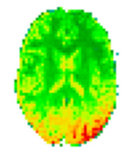
\includegraphics[width=0.1\textwidth]{fmri.png}};
        \node at ($(output)+(0,-1.3)$) {$\vec{x}_2$};
        
        
        \draw[-latex, line width=1pt, black!60] ($(x)+(0.2,0)$) -- ($(channel_organization)+(-0.25,0)$);
        \draw[-latex, line width=1pt, black!60] ($(channel_organization)+(0.2,0)$) -- ($(T)+(-0.2,0)$);
        \draw[-latex, line width=1pt, black!60] ($(T)+(0.2,0)$) -- ($(resblock1)+(-0.2,0)$);
        \draw[-latex, line width=1pt, black!60] ($(resblock1)+(0.2,0)$) -- ($(resblock2)+(-0.2,0)$);
        \draw[-latex, line width=1pt, black!60] ($(resblock2)+(0.2,0)$) -- ($(latent_affine)+(-0.2,0)$);
        \draw[-latex, line width=1pt, black!60] ($(latent_affine)+(0.25,0)$) -- ($(latent)+(-0.25,0)$);
        \draw[-latex, line width=1pt, black!60] ($(latent)+(0.25,0)$) -- ($(fourier)+(-1.25,0)$);
        \draw[-latex, line width=1pt, black!60] ($(fourier)+(1.25,0)$) -- ($(style)+(-0.25,0)$);
        \draw[-latex, line width=1pt, black!60] ($(style)+(0.25,0)$) -- ($(decoder_affine)+(-0.25,0)$);
        \draw[-latex, line width=1pt, black!60] ($(decoder_affine)+(0.25,0)$) -- ($(output)+(-0.8,0)$);
        \draw[-latex, line width=2pt, red!60] ($(style_weight)+(0,-0.25)$) -- ($(style)+(0,0.25)$);
        
        \node (attention_legend) at ($(encoder)+(-3.5,-3.4)$) {\tikz {\draw[draw=blue!50,fill=blue!20,thick] (0,0) rectangle ++(0.3,2);}};
        \node (resblock_legend) at ($(attention_legend)+(2.5,0)$) {\tikz {\draw[rounded corners, draw=red!40,fill=red!20,thick] (0,0) rectangle ++(0.3,2);}};
        \node (affine_legend) at ($(resblock_legend)+(3,0)$) {\tikz {\draw[draw=orange!40,fill=orange!20,thick] (0,0) rectangle ++(0.3,2);}};
        \node (hadamard_legend) at ($(affine_legend)+(3.8,0)$) {$\odot$};

        \node[align=left] at ($(affine_legend)+(1.7,0)$) {Affine projection};
        \node[align=left] at ($(attention_legend)+(1.1,0)$) {Attention};
        \node[align=left] at ($(resblock_legend)+(1.4,0)$) {Resnet block};
        \node at ($(hadamard_legend)+(2.,0)$) {Hadamard product};
        
    \end{tikzpicture}
    \caption{\textbf{Architecture of the CNN-TAG synthesizer.} The neural architecture has two components: an Encoder (shaded in grey) and a Decoder (shaded in green). The input is the STFT $v_1$ representation. The output is the synthesized fMRI. The Encoder begins with a simple attention mechanism on the channels dimension of the STFT. After, it is processed by two Resnet blocks and an affine layer. This produces the latent representation $\vec{z}$. Following, the Decoder picks this representation and builds the cosine bases through the projection $\omega \cdot \vec{z} + \beta$. The sinusoids are style induced with $cos(\omega \cdot \vec{z} + \beta)\odot W$. The vector $W$ is a style fixed pretrained vector of an fMRI representation, learned from a simultaneous EEG and fMRI dataset (described in Section \ref{section:fmri_data}). Finally, an affine layer projects it to the fMRI space.}
    \label{fig:horizontal_architecture}
\end{figure*}

The first synthesizer is the network introduced and validated in our earlier work \cite{calhas2022eeg}; its architecture is adopted from that study, not proposed here, and the present work re-implements it in PyTorch and retrains it with the protocol of Section~\ref{section:fmri_data}. We refer to it as CNN-TAG. Its flow is illustrated in Figure \ref{fig:horizontal_architecture}. Its input is the STFT view, $\vec{x}_1$; its output is the synthesized-fMRI view, $\vec{x}_2 \in \mathbb{R}^{M_1 \times M_2 \times M_3}$, a volume of $64\times64\times30$ voxels. The synthesized-fMRI view is therefore the composition $v_2 = F \circ v_1$ of the STFT transform and the network $F$.

In terms of structure, the network processes the input with an attention mechanism over channels. An attention weight matrix $A \in \mathbb{R}^{C \times (F T)}$ is used to compute $E \in \mathbb{R}^{C \times C}$, $E_{ij} = \vec{x}_i^\top A_j$, which is normalised with sparsemax along $j$ to give $B$; the attention-processed representation is
\begin{equation}\label{equation:attention_output}
    T_i  = \sum_j^C b_{ij}\, \vec{x}_j, \forall i \in \{1, \dots, C\}.
\end{equation}
$T$ is processed by two residual blocks \cite{he2016deep} and a fully connected layer, whose parameters $\theta_E$ form the encoder. The encoder output projects random Fourier features \cite{rahimi2007random,tancik2020fourier}, parameterized by $\omega$ and $\beta$ and layer-normalised around $\pi/2$; the resulting sinusoids are multiplied with a learned latent style vector, $W \in \mathbb{R}^L$, and an affine transformation maps them to the fMRI volume space. With this, we formulate the function structure $F: \mathbb{R}^{C \times F \times T} \to \mathbb{R}^{D_2}$.

\noindent\textbf{Other synthesizers.} Three published synthesizers were trained with the same data and protocol, using the authors' model code: \textbf{E2fNet} \cite{roos2025brainwaves}, a convolutional EEG encoder followed by a 2D U-Net and a convolutional fMRI decoder; \textbf{Spec2VolCAMU-Net} \cite{he2025spec2vol}, a multi-scale convolutional spectrogram encoder with temporal self-attention and a Vision-Mamba U-Net decoder, whose selective scan we computed with an exact pure-PyTorch chunked recurrence because the CUDA kernel was unavailable; and \textbf{NT-ViT} \cite{lanzino2024ntvit}, a mel-spectrogram vision-transformer encoder and decoder with a domain-matching loss, which computes its own spectrograms and therefore received the same 43.2\,s window as raw waveforms (the published model used a simultaneous 2.16\,s window without haemodynamic lag). CATD \cite{yao2025catd} could not be included because no code is available; NeuroBOLT and UnEBOLT \cite{li2024neurobolt,li2026unebolt} predict parcel time series rather than volumes and were used in the supporting fidelity analyses only.

\noindent\textbf{Untrained controls.} For each synthesizer, the same architecture with random initial weights was passed through the identical pipeline. A fixed nonlinear projection of EEG spectra into a voxel grid can support classification on its own; this control separates that effect from the learned EEG-to-fMRI mapping.

\noindent\textbf{Synthesizer training.} The synthesis target is the raw EPI volume min--max scaled to $[0,1]$ per volume, the convention of the published volumetric synthesizers. Synthesizers used for classification were trained on 14 NODDI subjects, with two subjects held out to select the training epoch; loss $0.5(1-\mathrm{SSIM})+0.5\,\mathrm{MSE}$, Adam, learning rate $10^{-3}$, batch size 32, mini-batches shuffled across subjects, 50 epochs (15 for Spec2VolCAMU-Net). NT-ViT used the authors' recipe (AdamW, learning rate $5\times10^{-4}$, 30 epochs) with batch size 32 instead of 128, because the 43.2\,s input did not fit in memory at 128. Input features were standardised with training-subject statistics only. The epoch with the highest validation SSIM was kept: epoch 11 for E2fNet, 10 for Spec2VolCAMU-Net and 20 for NT-ViT, but the first epoch (one pass over the training volumes) for CNN-TAG, whose validation SSIM did not improve afterwards (the same happened in 83 of its 96 leave-one-subject-out runs). Because a model selected after one epoch is close to its initialisation, CNN-TAG was also trained for all 50 epochs without selection and evaluated as a sensitivity analysis. NODDI carries no diagnostic labels and is never used for classification.

\noindent\textbf{Second training dataset (XP1).} To test whether the results depend on the training data, all four synthesizers were retrained on a second simultaneous EEG-fMRI dataset, XP1 (OpenNeuro ds002336) \cite{lioi2020xp}: ten healthy adults, 3\,T, TR 2\,s, 32 slices of 4\,mm, 64-channel MR-compatible EEG (BrainCap MR, the same layout as one NODDI montage, so the 57 channels are present by name), four runs each of motor imagery, neurofeedback and a motor localiser. We used the released gradient- and pulse-corrected EEG and matched each of its volume markers to a scanner trigger of the raw recording, anchored on the task markers present in both and validated on all of them. Because the number of raw triggers differed from the number of volumes in 15 of the 35 runs (one extra or up to six missing), only the 19 runs with exactly one trigger per volume were used (all ten subjects, about 3,700 volumes). Volumes were resampled from $106\times106\times32$ to the $64\times64\times30$ grid of NODDI, and EEG went through the same harmonisation, so the clinical inputs are unchanged. Eight subjects were used for training and two to select the epoch, with the NODDI training settings.

\noindent\textbf{From synthesized volumes to a subject view.} For each clinical subject, the synthesized volumes (one per pseudo-TR, clipped to $[0,1]$) are summarised by their voxelwise temporal mean and standard deviation, giving $2\times64\times64\times30$ features; this is the synthesized-fMRI view classified in Section~\ref{section:setting}.

\subsection{Contrastive sinusoid separation}\label{methods:separation}

In addition to the four synthesizers, we evaluate the integration approach of the earlier version of this work, which adapts the CNN-TAG synthesizer to the diagnostic task by separating classes in its sinusoid space while the voxel decoder is kept fixed.

CNN-TAG passes its encoder output $\vec{z}$ through random Fourier features, $\cos(\omega\cdot\vec{z}+\beta)$. Because the cosine is periodic, classes separated in $\vec{z}$ can overlap after the projection. The method therefore layer-normalises \cite{ba2016layer} $\vec{z}$ around $\pi/2$ with standard deviation $\pi/2$, which places most projections in an interval where the cosine is monotonic, and trains the encoder with the contrastive loss
\begin{equation}\label{equation:contrastive}
    \mathcal{L}_D(p_1, p_2, y_p) = y_p\, D(p_1, p_2) + (1-y_p)\, \left| D(p_1,p_2)-m \right|,
\end{equation}
where $p_1, p_2$ formulate a pair of two instances and $y_p \in \{0,1\}$ defines the pairwise label, being $0$ when the label of $p_1, p_2$ mismatch and $1$ when they match. $D(p_1,p_2) = \|p_1-p_2\|_1$ is the $l_1$ distance between the latent vectors of the pair, and $m \in (0, \pi]$ is the margin. Mismatched pairs are pulled to distance $m$ by an absolute deviation rather than pushed beyond it by a hinge, $\max(0, m - D)$, as in the original formulation: with the layer normalisation, this keeps the latent coordinates of both classes inside one non-periodic interval of the cosine, whereas a hinge lets distances grow past $\pi$, where the cosine wraps and the classes overlap again after projection (Additional file~1, Fig.~S1). Under the random projection, the expected similarity of two projected points decreases exponentially with their latent distance, so a margin that separates the classes in $\vec{z}$ also separates them after projection; Additional file~1 gives the statement, its proof and an illustration of the periodicity problem. Figure~\ref{fig:sinusoid_separation} illustrates the effect before and after training.

\noindent\textbf{Training.} The encoder is trained with $\mathcal{L}_D$ on pairs of EEG windows, while a linear classifier with an $l_1$ penalty is trained with $\mathcal{L}_C$ on the synthesized volume (detached from the encoder); the style vector and the voxel decoder stay frozen at their NODDI weights. Each synthesized window is an instance, and a subject's score is the mean predicted probability over its windows. We run two variants: \emph{re-initialised}, in which the encoder and Fourier projection start from random weights while the decoder keeps its NODDI weights, as in the original formulation, and \emph{pretrained}, in which they start from the NODDI-trained synthesizer and are fine-tuned. Training uses a fixed budget (10 epochs, Adam, learning rate $10^{-3}$, batches of 16 pairs, $l_1$ weight $10^{-4}$), without per-fold tuning.

\begin{figure}[ht]
    \centering
    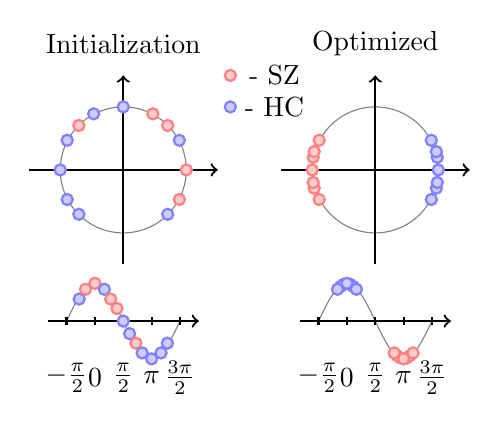
\begin{tikzpicture}
        [scale=0.8,
        inner sep=0.5mm,
        pd/.style={circle,draw=red!50,fill=red!20,thick},
        hc/.style={circle,draw=blue!50,fill=blue!20,thick}]
        
        %draw unit circle
        \node (uni_circle1) at (0,0) {};
        \draw[black!50, thin] ($(uni_circle1)$) circle [radius=1];
        \draw[black, thick, ->] ($(uni_circle1)+(-1.5,0)$) -- ($(uni_circle1)+(1.5,0)$);%xaxis
        \draw[black, thick, ->] ($(uni_circle1)+(0,-1.5)$) -- ($(uni_circle1)+(0,1.5)$);%yaxis
        
        \node (ind1) at ($(uni_circle1)+(1,0)$) [pd] {};
        \node (ind2) at ($(uni_circle1)+(0,1)$) [hc] {};
        \node (ind1) at ($(uni_circle1)+(-0.705,0.705)$) [pd] {};
        \node (ind1) at ($(uni_circle1)+(0.705,0.705)$) [pd] {};
        \node (ind1) at ($(uni_circle1)+(0.47,0.89)$) [pd] {};
        \node (ind2) at ($(uni_circle1)+(-1,0)$) [hc] {};
        \node (ind2) at ($(uni_circle1)+(-0.89,-0.47)$) [hc] {};
        \node (ind2) at ($(uni_circle1)+(-0.705,-0.705)$) [hc] {};
        \node (ind2) at ($(uni_circle1)+(0.89,0.47)$) [hc] {};
        \node (ind2) at ($(uni_circle1)+(-0.89,0.47)$) [hc] {};
        \node (ind2) at ($(uni_circle1)+(-0.47,0.89)$) [hc] {};
        \node (ind2) at ($(uni_circle1)+(0.89,-0.47)$) [pd] {};
        \node (ind2) at ($(uni_circle1)+(0.705,-0.705)$) [hc] {};
        
        
        \node (legend) at ($(uni_circle1)+(1.7,1)$) {};
        \node at ($(legend)+(0.7,0.5)$) {- SZ};
        \node at ($(legend)+(0.7,0)$) {- HC};
        \node at ($(legend)+(0,0.5)$) [pd] {};
        \node at ($(legend)+(0,0)$) [hc] {};
        
        %draw unit circle
        \node (uni_circle2) at ($(uni_circle1)+(4,0)$) {};
        \draw[black!50, thin] ($(uni_circle2)$) circle [radius=1];
        \draw[black, thick, ->] ($(uni_circle2)+(-1.5,0)$) -- ($(uni_circle2)+(1.5,0)$);%xaxis
        \draw[black, thick, ->] ($(uni_circle2)+(0,-1.5)$) -- ($(uni_circle2)+(0,1.5)$);%yaxis
        
        
        %individuals
        \node (ind1) at ($(uni_circle2)+(-1,0)$) [pd] {};
        \node (ind1) at ($(uni_circle2)+(-0.89,0.47)$) [pd] {};
        \node (ind1) at ($(uni_circle2)+(-0.985,0.2)$) [pd] {};
        \node (ind1) at ($(uni_circle2)+(-0.97,0.29)$) [pd] {};
        \node (ind1) at ($(uni_circle2)+(-0.89,-0.47)$) [pd] {};
        \node (ind1) at ($(uni_circle2)+(-0.97,-0.29)$) [pd] {};
        \node (ind1) at ($(uni_circle2)+(-0.985,-0.2)$) [pd] {};
        
        \node (ind2) at ($(uni_circle2)+(1,0)$) [hc] {};
        \node (ind1) at ($(uni_circle2)+(0.89,0.47)$) [hc] {};
        \node (ind1) at ($(uni_circle2)+(0.985,0.2)$) [hc] {};
        \node (ind1) at ($(uni_circle2)+(0.97,0.29)$) [hc] {};
        \node (ind1) at ($(uni_circle2)+(0.89,-0.47)$) [hc] {};
        \node (ind1) at ($(uni_circle2)+(0.97,-0.29)$) [hc] {};
        \node (ind1) at ($(uni_circle2)+(0.985,-0.2)$) [hc] {};
        
        
        
        \node (sinusoid1) at ($(uni_circle1)+(0,-2.7)$) {};
        \draw[black, thick, ->] ($(sinusoid1)+(-1.2,0.3)$) -- ($(sinusoid1)+(1.2,0.3)$);%xaxis
        \draw[thin, black!50] ($(sinusoid1)+(0.9,0.3)$) sin ($(sinusoid1)+(0.45,-0.3)$);
        \draw[thin, black!50] ($(sinusoid1)+(0.45,-0.3)$) cos ($(sinusoid1)+(0.,0.3)$);
        \draw[thin, black!50] ($(sinusoid1)+(0.,0.3)$) sin ($(sinusoid1)+(-0.45,0.9)$);
        \draw[thin, black!50] ($(sinusoid1)+(-0.45,0.9)$) cos ($(sinusoid1)+(-0.9,0.3)$);
        
        \draw[black, thick] ($(sinusoid1)+(-0.9,0.36)$) -- ($(sinusoid1)+(-0.9,0.24)$);
        
        \draw[black, thick] ($(sinusoid1)+(-0.45,0.36)$) -- ($(sinusoid1)+(-0.45,0.24)$);
        \draw[black, thick] ($(sinusoid1)+(0.,0.36)$) -- ($(sinusoid1)+(0.,0.24)$);
        \draw[black, thick] ($(sinusoid1)+(0.45,0.36)$) -- ($(sinusoid1)+(0.45,0.24)$);
        \draw[black, thick] ($(sinusoid1)+(0.9,0.36)$) -- ($(sinusoid1)+(0.9,0.24)$);
        
        \node at ($(sinusoid1)+(-0.9,-0.6)$) {$-\frac{\pi}{2}$};
        \node at ($(sinusoid1)+(-0.45,-0.6)$) {$0$};
        \node at ($(sinusoid1)+(0.,-0.6)$) {$\frac{\pi}{2}$};
        \node at ($(sinusoid1)+(0.45,-0.6)$) {$\pi$};
        \node at ($(sinusoid1)+(0.9,-0.6)$) {$\frac{3\pi}{2}$};
        
        \node (ind1) at ($(sinusoid1)+(-0.7,0.65)$) [hc] {};
        \node (ind1) at ($(sinusoid1)+(-0.6,0.805)$) [pd] {};
        \node (ind1) at ($(sinusoid1)+(-0.45,0.9)$) [pd] {};
        \node (ind1) at ($(sinusoid1)+(-0.3,0.805)$) [hc] {};
        \node (ind1) at ($(sinusoid1)+(-0.2,0.65)$) [pd] {};
        \node (ind1) at ($(sinusoid1)+(-0.1,0.5)$) [pd] {};
        \node (ind1) at ($(sinusoid1)+(0.,0.3)$) [hc] {};
        \node (ind1) at ($(sinusoid1)+(0.1,0.1)$) [hc] {};
        \node (ind1) at ($(sinusoid1)+(0.2,-0.05)$) [pd] {};
        \node (ind1) at ($(sinusoid1)+(0.3,-0.205)$) [hc] {};
        \node (ind1) at ($(sinusoid1)+(0.45,-0.3)$) [hc] {};
        \node (ind1) at ($(sinusoid1)+(0.6,-0.205)$) [hc] {};
        \node (ind1) at ($(sinusoid1)+(0.7,-0.05)$) [hc] {};
        
        \node (sinusoid2) at ($(uni_circle2)+(0,-2.7)$) {};
        \draw[black, thick, ->] ($(sinusoid2)+(-1.2,0.3)$) -- ($(sinusoid2)+(1.2,0.3)$);%xaxis
        \draw[thin, black!50] ($(sinusoid2)+(0.9,0.3)$) sin ($(sinusoid2)+(0.45,-0.3)$);
        \draw[thin, black!50] ($(sinusoid2)+(0.45,-0.3)$) cos ($(sinusoid2)+(0.,0.3)$);
        \draw[thin, black!50] ($(sinusoid2)+(0.,0.3)$) sin ($(sinusoid2)+(-0.45,0.9)$);
        \draw[thin, black!50] ($(sinusoid2)+(-0.45,0.9)$) cos ($(sinusoid2)+(-0.9,0.3)$);
        
        \draw[black, thick] ($(sinusoid2)+(-0.9,0.36)$) -- ($(sinusoid2)+(-0.9,0.24)$);
        
        \draw[black, thick] ($(sinusoid2)+(-0.45,0.36)$) -- ($(sinusoid2)+(-0.45,0.24)$);
        \draw[black, thick] ($(sinusoid2)+(0.,0.36)$) -- ($(sinusoid2)+(0.,0.24)$);
        \draw[black, thick] ($(sinusoid2)+(0.45,0.36)$) -- ($(sinusoid2)+(0.45,0.24)$);
        \draw[black, thick] ($(sinusoid2)+(0.9,0.36)$) -- ($(sinusoid2)+(0.9,0.24)$);
        
        \node at ($(sinusoid2)+(-0.9,-0.6)$) {$-\frac{\pi}{2}$};
        \node at ($(sinusoid2)+(-0.45,-0.6)$) {$0$};
        \node at ($(sinusoid2)+(0.,-0.6)$) {$\frac{\pi}{2}$};
        \node at ($(sinusoid2)+(0.45,-0.6)$) {$\pi$};
        \node at ($(sinusoid2)+(0.9,-0.6)$) {$\frac{3\pi}{2}$};
        
        
        \node (ind1) at ($(sinusoid2)+(-0.5,0.885)$) [hc] {};
        \node (ind1) at ($(sinusoid2)+(-0.55,0.85)$) [hc] {};
        \node (ind1) at ($(sinusoid2)+(-0.6,0.805)$) [hc] {};
        \node (ind1) at ($(sinusoid2)+(-0.4,0.885)$) [hc] {};
        \node (ind1) at ($(sinusoid2)+(-0.35,0.85)$) [hc] {};
        \node (ind1) at ($(sinusoid2)+(-0.3,0.805)$) [hc] {};
        \node (ind1) at ($(sinusoid2)+(-0.45,0.9)$) [hc] {};
        
        
        \node (ind1) at ($(sinusoid2)+(0.5,-0.285)$) [pd] {};
        \node (ind1) at ($(sinusoid2)+(0.55,-0.25)$) [pd] {};
        \node (ind1) at ($(sinusoid2)+(0.6,-0.205)$) [pd] {};
        \node (ind1) at ($(sinusoid2)+(0.4,-0.285)$) [pd] {};
        \node (ind1) at ($(sinusoid2)+(0.35,-0.25)$) [pd] {};
        \node (ind1) at ($(sinusoid2)+(0.3,-0.205)$) [pd] {};
        \node (ind1) at ($(sinusoid2)+(0.45,-0.3)$) [pd] {};
        
        \node (title1) at ($(uni_circle1)+(0,2)$) {Initialization};
        \node (title2) at ($(uni_circle2)+(0,2)$) {Optimized};
        
        %\node (stats1) at ($(uni_circle1)+(0,-4)$) {$\mathbb{E}[f_x(x)]=\frac{\pi}{2}, \mbox{Var}[f_x(x)]=\frac{\pi}{2}$};
        %\node (stats2) at ($(uni_circle2)+(0,-4)$) {$\mathbb{E}[f_x(x)]=\frac{\pi}{2}, \mbox{Var}[f_x(x)]=\frac{\pi}{2}$};
        
    \end{tikzpicture}
    \caption{\textbf{Contrastive separation of sinusoids.} Normalization of data points inside the unit circle, using layer normalization, along with the optimization of a contrastive loss lead to correct separation of sinusoids. Data points belong to two classes, $HC$ and $SZ$, that are separated after the minimization of $\mathcal{L}_D$. Because we separate false pairs, according to $(1-y_p) \times ||D(x_1,x_2)-m||_1$, all points are placed within a shift variant interval of the cosine. This preserves the between-class variance that the classifier needs.}
    \label{fig:sinusoid_separation}
\end{figure}

\subsection{Classification and statistical analysis}\label{section:setting}

The experiments compare, per cohort, the following views, each classified with an $l_2$-regularised logistic regression (Equation~\ref{equation:loss}), a linear classifier that allows a direct assessment of representational discriminative power and easy interpretation \cite{treviso2020explanation}:
(i) EEG-only views: the band-power view $v_0$ (relative log power); absolute log band power; and two views matched in information to the synthesized view, namely the temporal mean and standard deviation over pseudo-TRs of the synthesizers' own input spectra ($57$ channels $\times$ $97$ bins, $v_1^{\mathrm{ms}}$), and the same summary of a sparse random projection \cite{li2006sparse} to 8,192 dimensions of each pseudo-TR's complete $57\times97\times20$ input, an untrained linear map of exactly the information a synthesizer receives;
(ii) the synthesized-fMRI view $v_2$ of each synthesizer, reduced to 20 principal components, and the same view from the untrained synthesizers;
(iii) the combinations $v_0 \oplus v_2$ and $v_1^{\mathrm{ms}} \oplus v_2$, each high-dimensional block reduced by its own 20 components;
(iv) the contrastive sinusoid-separation classifier of Section~\ref{methods:separation} (two variants).
Sensitivity analyses repeat the classification with 5, 10 and 40 components; with synthesized volumes average-pooled in blocks of $3\times4\times4$ voxels; with covariates regressed out of every feature within training folds (age and sex in every cohort, chlorpromazine-equivalent dose in the psychosis cohorts, recording hour in Semmelweis and Fribourg, recording year in Fribourg); and with the ICA-cleaned inputs and, in Parkinson's disease, the rest-only crop of Section~\ref{section:adaptation}. All transformations (standardisation, covariate regression, principal components) are fitted on training folds only; principal components of high-dimensional blocks are computed exactly from the subject Gram matrix. Synthesis ran on NVIDIA A100, H100 and L4 GPUs and the linear models on CPU nodes.

\subsubsection{Validation}\label{section:validation}

To validate each view $v_i$, we perform repeated stratified 10-fold cross-validation at the subject level (20 repeats; 3 for the contrastive classifier), with one recording per person, and select the regularisation strength $C \in \{10^{-3},10^{-2},10^{-1},1,10\}$ by inner stratified 5-fold cross-validation within each training fold (Algorithm~\ref{alg:nested-cv}). We report the AUC averaged over repeats with a 95\% bootstrap confidence interval, obtained by resampling subjects (2,000 stratified resamples) with their repeat-averaged out-of-fold probabilities, and a one-sided label-permutation $p$-value, $p=(1+\#\{\mathrm{AUC}_{\mathrm{perm}}\geq\mathrm{AUC}\})/(1+N)$. Each permutation re-runs the complete nested procedure with two repeats; the null is therefore slightly wider than that of the 20-repeat estimate, which makes the test conservative. $N=1{,}000$ for the EEG views and 500 for the synthesized views (minimum $p\approx0.001$ and $0.002$); for the contrastive classifier, whose every permutation retrains the network, $N=20$ (minimum $p\approx0.048$), and its $p$-values are treated as exploratory. The added value of synthesis is $\Delta\mathrm{AUC}=\mathrm{AUC}(v_0\oplus v_2)-\mathrm{AUC}(v_0)$, and likewise relative to $v_1^{\mathrm{ms}}$. It is estimated with a paired stratified bootstrap over subjects (20,000 resamples), which gives a percentile 95\% interval, percentile intervals at the Bonferroni levels and a two-sided bootstrap $p$-value; $p$-values are Holm-adjusted within the family of the 20 trained-synthesizer comparisons (four synthesizers, five cohorts) and, separately, within the 40 comparisons that include the untrained synthesizers. Leave-one-subject-out estimates are reported only as a sensitivity analysis: with weak features they are biased below chance, because the class balance of each training set mirrors the held-out label \cite{varoquaux2018}.

\begin{algorithm}[t]
\caption{Nested repeated cross-validation for view $v_i$}
\label{alg:nested-cv}
\begin{algorithmic}[1]
\Require individuals $S$ with labels $y$; view $v_i$; hyperparameter grid $\mathcal{H}$; $R$ repeats
\Ensure AUC, out-of-fold probabilities $P$
\For{$r = 1$ \textbf{to} $R$}
    \For{each stratified fold $(S_{\text{train}}, S_{\text{test}})$ of $S$} \Comment{10 folds, subject level}
        \State fit standardisation (and PCA) on $S_{\text{train}}$ only
        \State $h^\star \gets \arg\max_{h \in \mathcal{H}} \textsc{CV}_5(v_i, S_{\text{train}}, h)$ \Comment{inner folds within $S_{\text{train}}$}
        \State fit $v_i$ with $h^\star$ on $S_{\text{train}}$; $P_r[S_{\text{test}}] \gets v_i.\textsc{predict}(S_{\text{test}})$
    \EndFor
\EndFor
\State \Return $\frac{1}{R}\sum_r \textsc{AUC}(P_r, y)$, $\frac{1}{R}\sum_r P_r$
\end{algorithmic}
\end{algorithm}

\subsection{Supporting synthesis analyses}\label{setting:fidelity}

To interpret the classification results we characterise what the synthesizers learn on NODDI. (a) \emph{Image protocol}: leave-one-subject-out over the 16 subjects (two validation subjects per fold for model selection), scored with SSIM, RMSE and voxelwise temporal correlation against an EEG-free population template (the mean training volume), with trigger-aligned EEG, EEG paired from the file start, and ECG only. (b) \emph{Fair target}: BOLD motion-corrected (rigid registration, FSL), cleaned with the Friston-24 motion model and spike regressors for framewise displacement above 0.5\,mm \cite{friston1996,power2014}, high-passed at 0.01\,Hz, z-scored, smoothed (6\,mm) and averaged into the 48 Harvard-Oxford grey-matter parcels present in every subject plus the global signal; ridge regression from lagged band power or full spectra, and UnEBOLT \cite{li2026unebolt} with its pretrained EEG encoder \cite{jiang2024labram}, predicted the parcel time series of held-out subjects. Significance used circular-shift and cross-subject swap nulls on detrended predictions and targets, and IAAFT surrogates of the BOLD with model refitting \cite{schreiber1996,mehta2025time}.

\subsection{Ethics approval}\label{section:ethics}

This study is a secondary analysis of anonymised, publicly released data; no new data were collected. All original studies were approved by the responsible committees and obtained informed consent from participants, as reported by the data providers: NODDI, approval ID 4290/001 \cite{dataset_01}; first-episode psychosis datasets, University of Pittsburgh Institutional Review Board \cite{salisbury_ds003944,salisbury_ds003947}; Semmelweis dataset, Semmelweis University Regional and Institutional Committee of Science and Research Ethics, registration number 197/2015 \cite{racz2025}; Parkinson's disease dataset, University of New Mexico Office of the Institutional Review Board \cite{cavanagh_ds003490} (approval numbers are not reported by the providers of the Pittsburgh and New Mexico data); Fribourg dataset, approval ID 054/13-CER-FR \cite{dataset2022fribourg}. The analyses were carried out in accordance with the relevant guidelines and regulations and the Declaration of Helsinki.

\section{Results}\label{section:results}

\subsection{EEG-only views}\label{section:res_eeg}

Relative band power separated Parkinson's disease from controls (AUC $0.786$, 95\% CI $0.63$--$0.92$, $p=0.002$) but not the psychosis or schizophrenia cohorts (Table~\ref{tab:eeg}): FEP1 $0.620$ ($p=0.07$), FEP2 $0.646$ ($p=0.050$), Semmelweis $0.571$ ($p=0.19$), Fribourg $0.539$ ($p=0.36$). Pooling the two first-episode samples ($n=138$) lowered the AUC to $0.568$ ($p=0.14$): the spectral differences that separate patients within one sample do not carry over to the other, consistent with sample heterogeneity (the two samples were also recorded mostly at different sampling rates, 1 and 3\,kHz). The information-matched view, the temporal mean and standard deviation of the synthesizers' own input spectra, was the best single view in Parkinson's disease ($0.825$, $p=0.001$), and an untrained sparse random projection of the full synthesizer input did equally well ($0.823$). In the other cohorts neither exceeded band power (FEP1 $0.52$, FEP2 $0.57$, Semmelweis $0.54$, Fribourg $0.56$).

\begin{table}[!htbp]
    \centering
    \caption{AUC of the EEG-only views (mean over 20 repeats of stratified 10-fold cross-validation; one-sided permutation $p$ in parentheses, 1,000 permutations; the random projection was not permutation-tested).}
    \label{tab:eeg}
    \footnotesize\setlength{\tabcolsep}{4pt}
    \begin{tabular}{@{}l c c c c@{}}
        \hline
        & \multicolumn{2}{c}{Band power} & Information- & Random \\
        Cohort & relative & absolute & matched & projection \\
        \hline
        FEP1 & $0.62$ ($0.07$) & $0.57$ ($0.21$) & $0.52$ ($0.35$) & $0.54$ \\
        FEP2 & $0.65$ ($0.05$) & $0.57$ ($0.22$) & $0.57$ ($0.25$) & $0.60$ \\
        Semmelweis & $0.57$ ($0.19$) & $0.56$ ($0.22$) & $0.54$ ($0.26$) & $0.61$ \\
        PD & $0.79$ ($0.002$) & $0.77$ ($0.002$) & $0.83$ ($0.001$) & $0.82$ \\
        Fribourg & $0.54$ ($0.36$) & $0.64$ ($0.11$) & $0.56$ ($0.28$) & $0.52$ \\
        \hline
    \end{tabular}
\end{table}

\subsection{Synthesized views}\label{section:res_clf}

In Parkinson's disease three of the four trained synthesizers produced views that discriminated patients from controls (E2fNet $0.744$, $p=0.010$; Spec2VolCAMU-Net $0.694$, $p=0.040$; NT-ViT $0.672$, $p=0.024$; CNN-TAG $0.483$, $p=0.46$; Table~\ref{tab:clf}, Fig.~\ref{fig:results}), but none reached band power or the information-matched view, and the same architectures with random weights did as well ($0.69$--$0.74$, all $p\leq0.026$). In the psychosis and schizophrenia cohorts no trained synthesizer was significant; among the untrained ones, Spec2VolCAMU-Net in Semmelweis ($0.740$, $p=0.006$) and NT-ViT in FEP2 ($0.626$, $p=0.048$) were. CNN-TAG in FEP2 fell well below chance ($0.329$; Section~\ref{section:res_checks}).

\begin{figure}[!htbp]
    \centering
    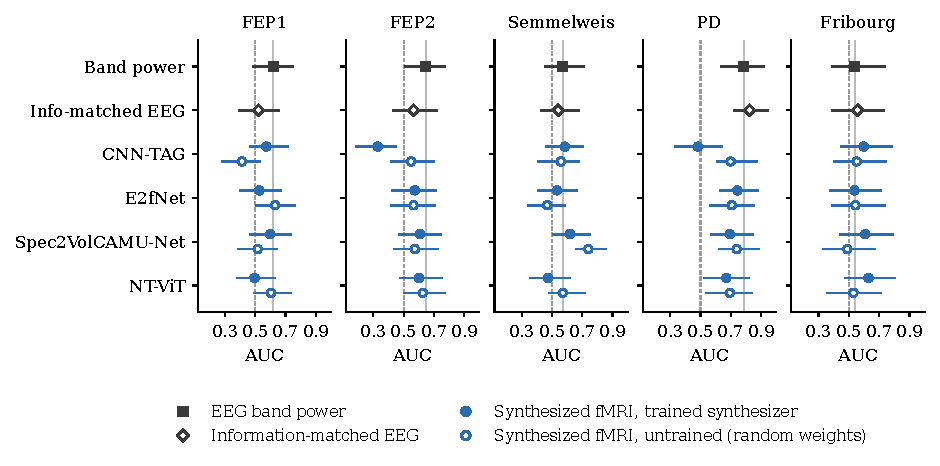
\includegraphics[width=\textwidth]{fig4.pdf}
    \caption{\textbf{Classification AUC by cohort and view.} Mean AUC over 20 repeats of stratified 10-fold cross-validation with 95\% bootstrap intervals, for EEG band power (squares), the information-matched EEG view (open diamonds) and the synthesized fMRI view of each synthesizer with learned weights (filled circles) or random weights (open circles). Dashed line: chance; grey line: band-power AUC. FEP1, FEP2: first-episode psychosis; Semmelweis: chronic schizophrenia; PD: Parkinson's disease; Fribourg: schizophrenia spectrum, task EEG.}
    \label{fig:results}
\end{figure}

\begin{table}[!htbp]
    \centering
    \caption{AUC of the synthesized-fMRI views of trained and untrained (random-weight) synthesizers (one-sided permutation $p$ in parentheses, 500 permutations).}
    \label{tab:clf}
    \footnotesize\setlength{\tabcolsep}{3pt}
    \begin{tabular}{@{}l l c c c c@{}}
        \hline
        Cohort & Weights & CNN-TAG & E2fNet & Spec2VolCAMU-Net & NT-ViT \\
        \hline
        FEP1 & trained & $0.57$ ($0.20$) & $0.53$ ($0.33$) & $0.60$ ($0.12$) & $0.50$ ($0.42$) \\
         & untrained & $0.41$ ($0.81$) & $0.63$ ($0.06$) & $0.52$ ($0.38$) & $0.60$ ($0.08$) \\
        FEP2 & trained & $0.33$ ($0.96$) & $0.57$ ($0.20$) & $0.61$ ($0.12$) & $0.60$ ($0.11$) \\
         & untrained & $0.55$ ($0.24$) & $0.57$ ($0.22$) & $0.57$ ($0.20$) & $0.63$ ($0.05$) \\
        Semmelweis & trained & $0.58$ ($0.14$) & $0.53$ ($0.28$) & $0.62$ ($0.06$) & $0.47$ ($0.64$) \\
         & untrained & $0.56$ ($0.17$) & $0.47$ ($0.59$) & $0.74$ ($0.006$) & $0.57$ ($0.12$) \\
        PD & trained & $0.48$ ($0.46$) & $0.74$ ($0.010$) & $0.69$ ($0.04$) & $0.67$ ($0.02$) \\
         & untrained & $0.70$ ($0.02$) & $0.71$ ($0.03$) & $0.74$ ($0.008$) & $0.69$ ($0.01$) \\
        Fribourg & trained & $0.60$ ($0.16$) & $0.54$ ($0.37$) & $0.61$ ($0.15$) & $0.63$ ($0.07$) \\
         & untrained & $0.55$ ($0.28$) & $0.54$ ($0.33$) & $0.49$ ($0.49$) & $0.53$ ($0.31$) \\
        \hline
    \end{tabular}
\end{table}

\subsection{Added value of synthesized fMRI}\label{section:res_delta}

Added to band power, no trained synthesizer gave a gain that survived Holm correction across the 20 comparisons (Table~\ref{tab:delta}). Nominal gains, with 95\% intervals excluding zero, occurred for Spec2VolCAMU-Net ($+0.035$) and NT-ViT ($+0.038$) in Parkinson's disease, E2fNet ($+0.067$) and Spec2VolCAMU-Net ($+0.112$) in Semmelweis, and E2fNet in Fribourg ($+0.075$), but adding the information-matched EEG view to band power gave a gain of the same size where the EEG carried signal (Parkinson's disease, $+0.030$, 95\% CI $+0.008$ to $+0.061$). Added to the information-matched view, no trained synthesizer improved classification in any cohort; the only difference that survived correction among trained synthesizers was a loss, for CNN-TAG in FEP2 ($-0.226$). Including the untrained synthesizers (40 comparisons per baseline), one gain survived Holm correction against both baselines: the untrained Spec2VolCAMU-Net in Semmelweis, $+0.165$ [$+0.089$, $+0.248$] over band power and $+0.169$ [$+0.073$, $+0.265$] over the information-matched view; the same network trained on NODDI added $+0.004$. Full-precision intervals, bootstrap $p$-values and Bonferroni-level intervals for all comparisons are given in Additional file~2.

\begin{table}[!htbp]
    \centering
    \caption{Added value of synthesized fMRI: $\Delta$AUC of the combined view over band power and over the information-matched EEG view, $^{*}$95\% paired bootstrap interval excludes zero; $^{\dagger}$Holm-adjusted $p<0.05$ across the 40 comparisons of trained and untrained synthesizers for that baseline. Intervals, bootstrap $p$-values and Bonferroni-level intervals are in Additional file~2.}
    \label{tab:delta}
    \scriptsize\setlength{\tabcolsep}{3pt}
    \begin{tabular}{@{}l l c c c c@{}}
        \hline
        & & \multicolumn{2}{c}{Over band power} & \multicolumn{2}{c}{Over information-matched EEG} \\
        Cohort & Synthesizer & Trained & Untrained & Trained & Untrained \\
        \hline
        FEP1 & CNN-TAG & $-0.042$ & $-0.095$$^{\dagger}$ & $-0.008$ & $-0.133$$^{*}$ \\
         & E2fNet & $+0.006$ & $-0.013$ & $-0.070$ & $+0.018$ \\
         & Spec2VolCAMU-Net & $-0.052$ & $+0.006$ & $+0.018$ & $-0.036$ \\
         & NT-ViT & $-0.028$ & $+0.018$ & $-0.044$ & $+0.055$ \\
        \hline
        FEP2 & CNN-TAG & $-0.024$ & $+0.028$ & $-0.226$$^{\dagger}$ & $-0.080$ \\
         & E2fNet & $-0.003$ & $+0.001$ & $-0.033$ & $-0.037$ \\
         & Spec2VolCAMU-Net & $+0.023$ & $+0.005$ & $+0.057$ & $-0.017$ \\
         & NT-ViT & $+0.012$ & $+0.001$ & $-0.015$ & $-0.009$ \\
        \hline
        Semmelweis & CNN-TAG & $+0.007$ & $+0.073$$^{*}$ & $+0.093$ & $+0.072$ \\
         & E2fNet & $+0.067$$^{*}$ & $-0.001$ & $+0.078$ & $+0.036$ \\
         & Spec2VolCAMU-Net & $+0.112$$^{*}$ & $+0.165$$^{\dagger}$ & $+0.004$ & $+0.169$$^{\dagger}$ \\
         & NT-ViT & $-0.013$ & $+0.096$$^{*}$ & $-0.021$ & $+0.026$ \\
        \hline
        PD & CNN-TAG & $+0.019$ & $+0.013$ & $-0.070$ & $-0.027$ \\
         & E2fNet & $+0.005$ & $+0.029$ & $-0.008$ & $-0.056$$^{*}$ \\
         & Spec2VolCAMU-Net & $+0.035$$^{*}$ & $-0.019$ & $+0.014$ & $-0.014$ \\
         & NT-ViT & $+0.038$$^{*}$ & $+0.027$ & $+0.006$ & $+0.024$ \\
        \hline
        Fribourg & CNN-TAG & $-0.000$ & $+0.002$ & $+0.018$ & $-0.029$ \\
         & E2fNet & $+0.079$$^{*}$ & $+0.061$$^{*}$ & $-0.029$ & $+0.004$ \\
         & Spec2VolCAMU-Net & $+0.013$ & $+0.042$ & $+0.009$ & $-0.013$ \\
         & NT-ViT & $-0.007$ & $+0.033$ & $+0.068$ & $-0.018$ \\
        \hline
    \end{tabular}
\end{table}

\subsection{Sensitivity analyses}\label{section:res_sens}

Table~\ref{tab:sens} compares, for each analysis, the best synthesized view (the maximum over the four synthesizers, which favours synthesis) with the information-matched EEG view. \textbf{Second training dataset.} Synthesizers retrained on XP1 reached AUC 0.34--0.68 across cohorts and synthesizers; none improved on the information-matched view (Additional file~2), and only Spec2VolCAMU-Net in Semmelweis ($0.66$) and in Parkinson's disease ($0.68$) were nominally significant. \textbf{Training length.} CNN-TAG trained for 50 epochs without epoch selection (validation SSIM $0.636$ against $0.686$ after the first epoch) reached $0.65$ in Parkinson's disease and $0.74$ in Semmelweis. \textbf{Dimensionality.} With 5, 10 or 40 components or block pooling, single synthesized views varied by up to $0.4$ AUC within a cohort (e.g.\ untrained E2fNet in Parkinson's disease, $0.34$ with 5 components and $0.77$ with 40), which shows how unstable they are at these sample sizes; no setting brought a trained synthesizer above the information-matched view. \textbf{Covariates.} Regressing out age and sex (and medication dose, recording hour or year where available) within training folds left Parkinson's disease unchanged (band power $0.80$, information-matched $0.83$), lowered FEP1 band power to $0.54$, and lowered the untrained Spec2VolCAMU-Net in Semmelweis from $0.74$ to $0.62$, so part of that effect follows age, sex or recording hour. \textbf{Artefacts.} Removing ocular components by ICA left Parkinson's disease unchanged (band power $0.81$, information-matched $0.80$) but lowered band power in FEP1 (from $0.62$ to $0.54$) and FEP2 (from $0.65$ to $0.58$), so part of the weak EEG signal of the first-episode cohorts was ocular. It also abolished the untrained Spec2VolCAMU-Net effect in Semmelweis ($0.57$, $p=0.13$); after ICA, no synthesized view gave a gain that survived Holm correction in any cohort (smallest adjusted $p=0.42$ over band power and $0.08$ over the information-matched view, 40 comparisons each); the only difference that survived among the trained synthesizers was a loss (Spec2VolCAMU-Net in FEP2, $-0.156$ relative to the information-matched view). Excluding the 30--45\,Hz band raised FEP1 band power to $0.73$ and left the other cohorts within $0.03$. In Parkinson's disease, restricting the analysis to the marked eyes-closed and eyes-open spans kept band power at $0.81$ ($0.82$ after ICA), so its discrimination is not carried by the set-up period, the oddball task or ocular artefacts; the information-matched view, whose temporal standard deviation rests on about 45 pseudo-TRs in this shorter crop, fell to $0.68$ ($0.75$ after ICA). In this crop the one-epoch CNN-TAG reached $0.81$ ($p=0.010$), above its untrained version ($0.57$), the only analysis in which a trained synthesizer clearly outperformed its random-weight control; it added nothing to band power ($+0.013$, 95\% CI $-0.018$ to $+0.045$), fell to $0.73$ after ICA, and its gain over the information-matched view ($+0.130$, 95\% CI $+0.003$ to $+0.270$, uncorrected $p=0.047$) did not survive Holm correction across the 16 comparisons of this analysis (adjusted $p\geq0.19$).

\begin{table}[!htbp]
    \centering
    \caption{Sensitivity analyses: AUC of the best synthesized view (syn., maximum over the four synthesizers, which favours synthesis) and of the information-matched EEG view (EEG) under the same analysis.}
    \label{tab:sens}
    \scriptsize\setlength{\tabcolsep}{2.5pt}
    \begin{tabular}{@{}l cc cc cc cc cc@{}}
        \hline
        & \multicolumn{2}{c}{FEP1} & \multicolumn{2}{c}{FEP2} & \multicolumn{2}{c}{Semmelweis} & \multicolumn{2}{c}{PD} & \multicolumn{2}{c}{Fribourg} \\
        Analysis & syn. & EEG & syn. & EEG & syn. & EEG & syn. & EEG & syn. & EEG \\
        \hline
        Primary (NODDI) & $0.60$ & $0.52$ & $0.61$ & $0.57$ & $0.62$ & $0.54$ & $0.74$ & $0.83$ & $0.63$ & $0.56$ \\
        Untrained & $0.63$ & $0.52$ & $0.63$ & $0.57$ & $0.74$ & $0.54$ & $0.74$ & $0.83$ & $0.55$ & $0.56$ \\
        Trained on XP1 & $0.63$ & $0.52$ & $0.57$ & $0.57$ & $0.66$ & $0.54$ & $0.68$ & $0.83$ & $0.54$ & $0.56$ \\
        CNN-TAG 50 epochs & $0.49$ & $0.52$ & $0.48$ & $0.57$ & $0.74$ & $0.54$ & $0.65$ & $0.83$ & $0.66$ & $0.56$ \\
        5--40 comp., pooling & $0.65$ & $0.52$ & $0.62$ & $0.57$ & $0.68$ & $0.54$ & $0.74$ & $0.83$ & $0.67$ & $0.56$ \\
        Covariates removed & $0.60$ & $0.52$ & $0.59$ & $0.55$ & $0.63$ & $0.53$ & $0.75$ & $0.83$ & $0.62$ & $0.49$ \\
        ICA (ocular) & $0.62$ & $0.55$ & $0.54$ & $0.54$ & $0.63$ & $0.49$ & $0.70$ & $0.80$ & $0.62$ & $0.65$ \\
        \hline
    \end{tabular}
\end{table}

\subsection{Recording conditions, artefacts and a below-chance estimate}\label{section:res_checks}

No recording metadata differed between groups in FEP1 or Parkinson's disease; in FEP2 the raw recordings of patients were longer (removed by the fixed crop). Semmelweis patients were recorded earlier in the day than controls (mean hour $14.0$ against $16.3$, $p<0.001$), and in Fribourg the nine participants recorded in 2016 were all patients and the auxiliary channel layout differed by group (Additional file~2). Artefact burden differed by group in two cohorts: in Parkinson's disease controls had larger EEG amplitudes and more ocular activity than patients (EOG power, AUC $0.26$, $p=0.004$), consistent with the reduced blink rate of Parkinson's disease, whereas accelerometer power did not differ ($p=0.28$); in Semmelweis patients had more high-amplitude segments ($p=0.003$). The number of ocular components removed by ICA did not differ between groups in any cohort (all $p\geq0.07$). In Parkinson's disease every recording followed the same order (one minute of eyes closed, then one minute of eyes open, then the oddball task), and the onsets of the rest spans and of the task did not differ between groups ($p=0.54$ and $p=0.31$); the fixed 0--400\,s crop of the primary analysis therefore included a variable set-up period before rest and the start of the oddball task.

The below-chance AUC of CNN-TAG in FEP2 is not explained by a nuisance factor: none of its first 20 principal components was associated with sampling rate, recording duration, age, sex or medication dose ($|\rho|\leq0.20$), and no subject carried more than $26\%$ of any of the first five. In every outer fold the inner cross-validation AUC was below $0.5$ ($0.35$--$0.44$) while the training AUC was $0.71$--$0.83$, the signature of anti-learning in features without signal: when the full-sample difference between groups is close to zero, the difference in a training fold is opposite to that in its held-out fold, so a fitted direction reverses out of sample \cite{varoquaux2018}.

\subsection{Contrastive sinusoid separation}\label{section:res_contrastive}

 The contrastive classifier discriminated only in Parkinson's disease, at the smallest attainable $p$, and stayed below band power there (Table~\ref{tab:contrastive}). Initialising the encoder from the NODDI-trained synthesizer did not improve on re-initialisation.

\begin{table}[!htbp]
    \centering
    \caption{Contrastive sinusoid separation: AUC (repeated stratified 10-fold, 3 repeats), 95\% bootstrap interval and permutation $p$ (20 permutations; minimum $0.048$).}
    \label{tab:contrastive}
    \footnotesize\setlength{\tabcolsep}{4pt}
    \begin{tabular}{@{}l c c c@{}}
        \hline
        \hline
        \hfil Cohort & \hfil Re-initialised encoder & \hfil Pretrained encoder & \hfil Band power \\
        \hline
        FEP1 & $0.485$ [$0.39$, $0.67$] ($0.57$) & $0.599$ [$0.48$, $0.73$] ($0.19$) & $0.620$ \\
        FEP2 & $0.476$ [$0.34$, $0.63$] ($0.52$) & $0.433$ [$0.27$, $0.54$] ($0.76$) & $0.646$ \\
        Semmelweis & $0.538$ [$0.46$, $0.72$] ($0.33$) & $0.562$ [$0.45$, $0.70$] ($0.24$) & $0.571$ \\
        PD & $0.701$ [$0.58$, $0.86$] ($0.048$) & $0.660$ [$0.53$, $0.82$] ($0.048$) & $0.786$ \\
        Fribourg & $0.559$ [$0.38$, $0.74$] ($0.33$) & $0.602$ [$0.44$, $0.77$] ($0.14$) & $0.539$ \\
        \hline
        \hline
    \end{tabular}
\end{table}

\subsection{What the synthesizers learn}\label{section:res_fidelity}

On NODDI, leave-one-subject-out over the 16 subjects (Table~\ref{tab:fidelity}), the EEG-free template (the mean training volume) reached SSIM $0.675$ and PSNR $21.2$; under E2fNet's own data pipeline, which pairs EEG and fMRI from the start of the file, the same template reached $0.676$ and $21.2$. Both are above the published SSIM of E2fNet ($0.605$) and NT-ViT ($0.581$) and slightly below that of Spec2VolCAMU-Net ($0.693$); the published values come from each study's own data split and preprocessing and are therefore indicative only. Retrained with trigger-aligned EEG, ridge regression, CNN-TAG and E2fNet were below the template on SSIM ($0.631$--$0.655$, Wilcoxon $p\leq0.003$ over subjects) and all four synthesizers were worse on RMSE ($p\leq0.0002$); Spec2VolCAMU-Net tied it on SSIM ($0.679$, higher in 11 of 16 subjects, $p=0.30$). Pairing EEG from the start of the file or replacing EEG by the ECG left these values almost unchanged, and no model showed a voxelwise temporal correlation above that obtained with circularly shifted EEG. The final synthesizers used for the clinical cohorts behaved the same on the two held-out NODDI subjects (SSIM within $0.03$ of the template, voxelwise $r\approx0$; Additional file~2), as did the synthesizers retrained on XP1 (SSIM $0.662$--$0.699$ against a template of $0.684$ on two held-out XP1 subjects). Figure~\ref{fig:examples} shows why: Spec2VolCAMU-Net and NT-ViT produce an almost constant, template-like volume (voxelwise temporal SD close to zero), E2fNet varies mainly at the brain edge, and the one-epoch CNN-TAG fluctuates more than the real data without following it. Between subjects, a synthesizer's output therefore differs mainly through the subject's overall EEG spectrum. With a target that removes anatomy and motion (Section~\ref{setting:fidelity}), EEG predicted a statistically detectable but negligible part of BOLD in held-out subjects: ridge regression from full spectra $r=0.026$, UnEBOLT $r=0.035$ (above shift and swap nulls, $p=0.02$ and $p=0.03$), with $R^2\approx0$ for both; within subjects, $r\approx0$.

\begin{table*}[!htbp]
    \centering
    \caption{Fidelity on NODDI, leave-one-subject-out (16 test subjects; mean $\pm$ SD over subjects, seeds averaged within a subject). PSNR from the RMSE of $[0,1]$-scaled volumes (RMSE in Additional file~2). $r$: mean voxelwise temporal correlation with the real volumes; shift null: the same with circularly shifted EEG. Epoch: median selected epoch.}
    \label{tab:fidelity}
    \scriptsize\setlength{\tabcolsep}{2.5pt}
    \begin{tabular}{@{}l l c c c c c@{}}
        \hline
        Input & Model & SSIM & PSNR & $r$ & $r$ (shift null) & Epoch \\
        \hline
        Aligned EEG & EEG-free template & $0.675\pm0.044$ & $21.2\pm1.2$ & $+0.000$ & -- & -- \\
         & Ridge (spectra) & $0.631\pm0.046$ & $19.9\pm1.2$ & $-0.001$ & $+0.000$ & -- \\
         & CNN-TAG & $0.655\pm0.048$ & $20.2\pm1.0$ & $+0.001$ & $-0.002$ & 0 \\
         & E2fNet & $0.655\pm0.053$ & $19.6\pm1.1$ & $-0.003$ & $+0.001$ & 10 \\
         & Spec2VolCAMU-Net & $0.679\pm0.052$ & $20.7\pm1.2$ & $-0.000$ & $+0.000$ & 13 \\
        File-start EEG & Ridge (spectra) & $0.631\pm0.046$ & $19.9\pm1.1$ & $-0.001$ & $-0.000$ & -- \\
         & CNN-TAG & $0.640\pm0.047$ & $20.0\pm1.2$ & $-0.004$ & $+0.000$ & 0 \\
         & E2fNet & $0.661\pm0.057$ & $19.8\pm1.2$ & $+0.002$ & $-0.000$ & 10 \\
        ECG only & Ridge (spectra) & $0.600\pm0.060$ & $19.4\pm1.4$ & $-0.000$ & $-0.001$ & -- \\
         & CNN-TAG & $0.650\pm0.046$ & $20.1\pm1.1$ & $-0.004$ & $+0.001$ & 0 \\
         & E2fNet & $0.648\pm0.056$ & $19.4\pm1.5$ & $-0.001$ & $+0.000$ & 10 \\
        \hline
    \end{tabular}
\end{table*}

\begin{figure*}[!htbp]
    \centering
    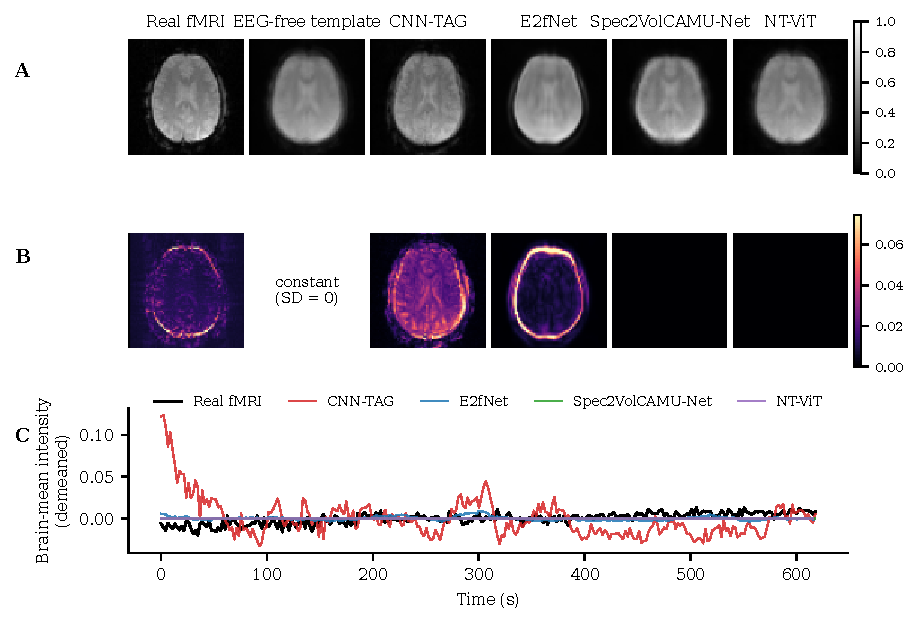
\includegraphics[width=\textwidth]{fig5.pdf}
    \caption{\textbf{Synthesized volumes of a held-out subject.} NODDI subject 49 (held out from training), final synthesizers used for the clinical cohorts. \textbf{A} One volume (axial slice 15 of 30) of the real data, the EEG-free template and each synthesizer. \textbf{B} Voxelwise temporal standard deviation over the 287 volumes (same scale for all). \textbf{C} Brain-mean intensity over time, demeaned, on the same intensity scale.}
    \label{fig:examples}
\end{figure*}

\section{Discussion}\label{section:discussion}

\noindent\textbf{Synthesized fMRI did not add diagnostic information beyond the EEG it is computed from.} Across four synthesizers trained on two simultaneous EEG-fMRI datasets and five clinical cohorts, no trained synthesizer improved classification over an EEG view that received the same spectral information, and none of their gains over band power survived correction for multiple comparisons. Where gains over band power occurred, adding the information-matched EEG view to band power gave gains of the same size, and where synthesized views discriminated patients from controls, most clearly in Parkinson's disease, the same architectures with random weights did as well. Retraining on a second dataset, training CNN-TAG to convergence, changing the dimensionality reduction and regressing out covariates did not change this.

\noindent\textbf{Representation, not information.} A synthesizer cannot add information absent from its input, and the case for synthesized fMRI in small clinical samples is therefore representational: a mapping learned from simultaneous recordings could reorganise EEG spectra into a space in which group differences are linearly accessible to a classifier trained on 50--80 subjects. The controls used here separate three possible sources of a gain: a richer EEG summary (the information-matched view), the inductive bias of the network architecture (the untrained networks) and the learned EEG-to-fMRI mapping (the difference between trained and untrained networks). Every gain we observed came from the first two; none came from the learned mapping. In one sensitivity analysis (Parkinson's disease, rest-only crop) a trained synthesizer did outperform its random-weight control, but it still added nothing to band power. The one gain that survived correction for 40 comparisons, the untrained Spec2VolCAMU-Net in chronic schizophrenia, looked like an architecture effect: a fixed, multi-scale, nonlinear projection of EEG spectra extracted a difference that linear summaries of the same spectra did not. It was also the least robust: it shrank when age, sex and recording hour were regressed out (patients were recorded earlier in the day), it disappeared when ocular components were removed by ICA (AUC $0.57$, $p=0.13$), and neither the NODDI- nor the XP1-trained Spec2VolCAMU-Net reproduced it. It most likely reflects ocular artefacts and recording conditions that differ between the groups of this cohort, not the disease and not synthesis.

\noindent\textbf{Why the learned mapping adds nothing.} Under the image protocol used by published synthesizers, the models reproduce the static anatomy that an EEG-free template already captures: Spec2VolCAMU-Net and NT-ViT produce an almost constant volume, and the outputs of all four synthesizers differ between subjects mainly through each subject's overall EEG spectrum. Their subject-level summaries are then nonlinear transforms of the same spectra that the information-matched view summarises linearly. Under a fair BOLD target, EEG predicts a statistically detectable but negligible share of the variance even with a state-of-the-art model. A synthesized volume therefore cannot yet carry haemodynamic information that would distinguish it from a transform of the EEG, and a diagnostic gain from the learned mapping would not be expected.

\noindent\textbf{Scope.} These conclusions concern current volumetric synthesizers trained on small simultaneous datasets of healthy adults (16 subjects at 1.5\,T, rest; 10 subjects at 3\,T, motor imagery and neurofeedback) and applied to clinical EEG that differs from the training data in recording system, montage, eye state and, in one cohort, paradigm. They do not exclude that EEG-to-fMRI synthesis, trained on larger or clinical simultaneous data and with an EEG-dependent mapping demonstrated in held-out subjects, could add diagnostic information. They do show that such a claim needs the controls of Table~\ref{tab:checklist} to be credible.

\noindent\textbf{Artefacts and recording conditions.} Three cohorts showed group differences unrelated to the disease process that a classifier can exploit: more ocular activity in controls than in patients with Parkinson's disease, consistent with reduced blinking in Parkinson's disease, but the discrimination of that cohort persisted after removing ocular components (band power AUC $0.81$; $0.82$ on rest-only data); ocular components also carried part of the weak signal of the first-episode cohorts (band power fell from $0.62$ to $0.54$ in FEP1 and from $0.65$ to $0.58$ in FEP2 after ICA) and all of the untrained-network gain in Semmelweis; earlier recording times and more high-amplitude segments in Semmelweis patients; and recording year and auxiliary channel layout in Fribourg. In Parkinson's disease, the commonly used rest file also contained a set-up period and the start of an auditory oddball task. None of these is visible in a classification table, and all of them would affect a synthesized view in the same way as the EEG it is computed from.

\noindent\textbf{A checklist for diagnostic claims.} Table~\ref{tab:checklist} lists the controls of the protocol, the alternative explanation each rules out and what it showed here. Two of them concern synthesis itself: the NODDI dataset, the most used benchmark for volumetric synthesis, requires pairing EEG and fMRI through the scanner markers and selecting channels by name, two steps invisible to SSIM and PSNR, which an EEG-free template already maximises. We recommend that synthesis studies report an EEG-free template and temporal metrics against shift and swap nulls, and that diagnostic uses of synthesized fMRI report an EEG-only baseline, untrained-network controls and checks for acquisition differences between groups. A synthesizer that passes these controls would provide the first evidence that synthesized fMRI adds diagnostic information; the released code implements them and can be applied to new synthesizers.

\begin{table}[!htbp]
    \centering
    \caption{Controls for diagnostic claims from synthesized fMRI: what each rules out and what it showed in this study.}
    \label{tab:checklist}
    \footnotesize
    \begin{tabular}{@{}>{\raggedright\arraybackslash}p{3.4cm}>{\raggedright\arraybackslash}p{4.0cm}>{\raggedright\arraybackslash}p{4.4cm}@{}}
        \hline
        Control & Alternative explanation ruled out & In this study \\
        \hline
        EEG-only baseline under identical validation & Synthesized fMRI adds nothing beyond the EEG it is computed from & Band power above every synthesized view in Parkinson's disease \\
        EEG view matched in information to the synthesizer input & The gain comes from a richer EEG summary, not from synthesis & Matched view the best single view in Parkinson's disease; no trained synthesizer added to it \\
        Fusion test, paired bootstrap, correction for multiplicity & Chance gains among many model--cohort comparisons & No trained-synthesizer gain survived Holm correction \\
        Untrained-network control & Discrimination by the architecture's inductive bias rather than the learned mapping & Untrained synthesizers matched trained ones in Parkinson's disease ($0.69$--$0.74$); the one robust gain came from an untrained network \\
        Channel selection by type; acquisition checks & Group differences in recording set-up & Auxiliary-channel layout and recording year (Fribourg) and time of day (Semmelweis) differed by group \\
        Artefact handling (ICA) and artefact measures by group & Discrimination by ocular, muscle or movement artefacts & Ocular activity differed by group in Parkinson's disease, whose discrimination persisted after ICA; the one robust gain (Semmelweis) disappeared after ICA \\
        A crop with the same content in every recording & Task or set-up periods in a resting-state analysis & The Parkinson's disease rest file contained a set-up period and an oddball task \\
        Subject-level nested cross-validation; permutation tests & Windows of one subject in training and test folds; tuning on test data; anti-learning bias of leave-one-out & All estimates subject-level with permutation $p$ \\
        EEG-free template image & Fidelity that reflects static anatomy & Template matched or exceeded all synthesizers (SSIM) \\
        Temporal metrics against shift and swap nulls & Fidelity unrelated to EEG timing & Voxelwise $r\approx0$; parcel $r\approx0.03$ on a fair BOLD target \\
        Trigger alignment and channels by name (NODDI) & EEG paired with the wrong volumes or electrodes & EEG starts 13--130\,s before the first volume in 15 of 16 subjects \\
        \hline
    \end{tabular}
\end{table}

\subsection{Limitations}\label{section:limitations}

Sample sizes are modest (43--77 subjects per cohort), so AUC intervals are wide and null results bound but do not exclude small effects; single synthesized views were also unstable across dimensionality-reduction settings. Resting EEG carried weak signal in the psychosis and schizophrenia cohorts, so the evaluation is most informative in Parkinson's disease. The synthesizers were trained on two small healthy datasets (Section~\ref{section:fmri_data}); for XP1, runs whose scanner triggers could not be matched one-to-one to volumes were excluded. The epoch selected for CNN-TAG was the first one, which we addressed by training it for 50 epochs. The clinical EEG differed from the training data in system, montage (interpolated), eye condition and paradigm, and no clinical cohort has paired fMRI, so synthesis fidelity in patients cannot be measured. Artefact handling was limited to ocular components: with a 45\,Hz low-pass the standard muscle criterion was not usable, so muscle artefacts were addressed only by excluding the 30--45\,Hz band, and an amplitude-based rejection threshold of 150\,$\mu$V would have removed most of the data and was used descriptively. Patients were medicated in the psychosis and schizophrenia cohorts; medication dose was regressed out where available. Each subject's synthesized sequence was summarised by its temporal mean and standard deviation; other summaries, such as synthesized connectivity, were not tested. The contrastive classifier used fixed hyperparameters and 20 permutations. CATD could not be evaluated, and NeuroBOLT and UnEBOLT were used for fidelity only.

\section{Conclusions}\label{section:conclusion}

We introduced a controlled protocol for testing whether EEG-synthesized fMRI aids diagnosis and applied it to four synthesizers, trained on two simultaneous EEG-fMRI datasets, and five public cohorts spanning first-episode psychosis, chronic schizophrenia and Parkinson's disease. No trained synthesizer added diagnostic information to an EEG view matched in the information it receives, untrained networks reproduced the discrimination of synthesized views, and the contrastive sinusoid-separation method did not change this; the one gain that survived correction came from an untrained network and disappeared after ocular artefacts were removed. Claims that synthesized fMRI aids diagnosis should therefore be tested against information-matched EEG baselines, untrained-network controls and recording-condition checks, and synthesizers should first show fidelity beyond an EEG-free template and EEG-timing nulls. The protocol, code and checklist are released so that future synthesizers can be evaluated in the same way. An extension of the contrastive formulation to more than two classes is sketched in Additional file~1.

\section*{List of abbreviations}
AUC: area under the receiver operating characteristic curve; BOLD: blood-oxygen-level-dependent; CI: confidence interval; CNN-TAG: convolutional neural network with topographical attention graph; ECG: electrocardiogram; EEG: electroencephalography; EMG: electromyogram; EOG: electrooculogram; EPI: echo-planar imaging; FEP: first-episode psychosis; fMRI: functional magnetic resonance imaging; IAAFT: iterative amplitude-adjusted Fourier transform; ICA: independent component analysis; MSE: mean squared error; PANSS: Positive and Negative Syndrome Scale; PD: Parkinson's disease; PSNR: peak signal-to-noise ratio; RMSE: root mean squared error; ROC: receiver operating characteristic; SSIM: structural similarity index measure; TR: repetition time.

\backmatter

\bmhead{Supplementary information}
\textbf{Additional file 1} (PDF). Supplementary methods: datasets and data checks (S1); pairing EEG and fMRI in NODDI and XP1, and synthesizer training (S2); EEG harmonisation and artefact handling (S3); EEG views and synthesizers, with the CNN-TAG architecture (S4, Fig.~S1); the contrastive sinusoid-separation method with its separation property, proof and multi-class extension (S5); classification and statistics, including the diagnostic of the below-chance CNN-TAG estimate in FEP2 (S6); and the fidelity and fair-target analyses (S7). \textbf{Additional file 2} (PDF). Supplementary tables: added value of synthesized fMRI at full precision, with bootstrap $p$-values, Bonferroni-level intervals and Holm adjustment (Table~S1); AUC of every view with intervals and permutation $p$ (Table~S2); recording metadata and artefact measures by group (Table~S3); the contrastive classifier (Table~S4); fidelity of the final and XP1-trained synthesizers on held-out subjects (Table~S5) and leave-one-subject-out fidelity on NODDI (Table~S6); sensitivity of each synthesized view (Table~S7).

\section*{Declarations}

\bmhead{Availability of data and materials}
All datasets analysed in this study are publicly available: NODDI simultaneous EEG-fMRI (Open Science Framework, \url{https://osf.io/94c5t}) \cite{dataset_01}; first-episode psychosis resting EEG, OpenNeuro ds003944 and ds003947 \cite{salisbury_ds003944,salisbury_ds003947}; Semmelweis schizophrenia resting EEG, Zenodo record 14808296 \cite{racz2025}; Parkinson's disease resting EEG, OpenNeuro ds003490 \cite{cavanagh_ds003490}; Fribourg Ultimatum Game EEG, OpenNeuro ds004000 \cite{dataset2022fribourg}; XP1 simultaneous EEG-fMRI, OpenNeuro ds002336 \cite{lioi2020xp}. No new data were collected. The code, and the derived results (classification outputs, fidelity summaries and the per-subject recording metadata used in the analyses), are available at \url{https://github.com/DCalhas/eeg_to_fmri} (branch \texttt{rebuild-2026}). Project name: eeg\_to\_fmri; operating system: Linux; programming language: Python; other requirements: PyTorch, MNE-Python, scikit-learn, FSL; licence: MIT.

\bmhead{Competing interests}
The authors declare that they have no competing interests.

\bmhead{Funding}
This work was supported by national funds through Funda\c{c}\~{a}o para a Ci\^{e}ncia e Tecnologia (FCT), under the Ph.D.\ Grant SFRH/BD/5762/2020 to David Calhas. This research was supported by the Slovenian Research and Innovation Agency (ARIS) under the Artificial Intelligence and Intelligent Systems Programme (Grant No.~P2-0209) and by the European project 22HLT05 MAIBAI. This publication is co-funded by the European Union's Horizon Europe research and innovation programme under the Marie Sk{\l}odowska-Curie COFUND Postdoctoral Programme grant agreement No.~101081355-SMASH and by the Republic of Slovenia and the European Union from the European Regional Development Fund. Views and opinions expressed are however those of the author(s) only and do not necessarily reflect those of the European Union or the European Research Executive Agency. Neither the European Union nor the granting authority can be held responsible for them.

\bmhead{Authors' contributions}
DC developed the code and the experiments. RH contributed to the supervision, the experimental setting and the revision of the manuscript. All authors read and approved the final manuscript.

\bmhead{Acknowledgements}
We thank the groups that collected and publicly released the datasets used in this study.

\bibliography{references}

\end{document}
